%%%%%%%%%%%%%%%%%%%%%%%%%%%%%%%%%%%%%%%%%%%%%%%%%%%%%%%%%%%%%%%%%%%%%%%%%%%%
%% CR-SHE
%% Prepared for Elsevier, Future Generation Computer Systems
%% Elsevier CAS double-column template (cas-dc)
%%
%% Build:  pdflatex -> bibtex -> pdflatex -> pdflatex
%%
%% House-style notes for this file
%%   * No em dashes anywhere in the text. Parenthetical asides use
%%     commas, colons, semicolons or parentheses instead. The double hyphen
%%     (--) appears only as an en dash inside numeric ranges, which is the
%%     Elsevier convention for ranges.
%%   * Fig. 1 (the architecture) is a full-text-width figure* float; it is
%%     regenerated by figures_src/fig_architecture.py.
%%%%%%%%%%%%%%%%%%%%%%%%%%%%%%%%%%%%%%%%%%%%%%%%%%%%%%%%%%%%%%%%%%%%%%%%%%%%

\documentclass[a4paper,fleqn]{cas-dc}

\usepackage[numbers,sort&compress]{natbib}
\usepackage{algorithm}
\usepackage{algpseudocode}

% Let a tight line stretch rather than spill into the neighbouring column.
\setlength{\emergencystretch}{3em}

% amssymb (loaded by cas-dc) supplies \checkmark; this is a harmless guard in
% case a future font package withdraws it.
\providecommand{\checkmark}{\ensuremath{\surd}}

% Theorem-like environments, using the constructs cas-dc provides.
\newtheorem{theorem}{Theorem}
\newtheorem{lemma}{Lemma}
\newdefinition{definition}{Definition}
\newdefinition{remark}{Remark}
\newproof{pf}{Proof}

\newcommand{\negl}{\mathsf{negl}}
\newcommand{\PPT}{\mathrm{PPT}}
\newcommand{\Real}{\mathbf{Real}}
\newcommand{\Ideal}{\mathbf{Ideal}}
\newcommand{\Leak}{\mathcal{L}}
\newcommand{\Sim}{\mathcal{S}}
\newcommand{\Adv}{\mathcal{A}}
\newcommand{\cind}{\approx_c}
\newcommand{\Gen}{\mathsf{Gen}}
\newcommand{\Eval}{\mathsf{Eval}}
\newcommand{\Setupp}{\mathsf{Setup}}
\newcommand{\BuildIndex}{\mathsf{BuildIndex}}
\newcommand{\EncData}{\mathsf{EncData}}
\newcommand{\Token}{\mathsf{Token}}
\newcommand{\Search}{\mathsf{Search}}
\newcommand{\Compute}{\mathsf{Compute}}
\newcommand{\Dec}{\mathsf{Dec}}
\newcommand{\Enc}{\mathsf{Enc}}
\newcommand{\advPRF}{\mathbf{Adv}^{\mathrm{prf}}}
\newcommand{\advDPF}{\mathbf{Adv}^{\mathrm{dpf}}}
\newcommand{\advCPA}{\mathbf{Adv}^{\mathrm{cpa}}}
\newcommand{\bplus}{\boxplus}
\newcommand{\bminus}{\boxminus}
\newcommand{\bdot}{\boxdot}

\begin{document}
\let\WriteBookmarks\relax
\def\floatpagepagefraction{1}
\def\textpagefraction{.001}

\shorttitle{Oblivious homomorphic aggregation for multi-cloud IoT analytics}
\shortauthors{M. M. Islam et~al.}

\title[mode=title]{CR-SHE: Oblivious homomorphic aggregation for
collusion-resilient search and analytics over encrypted multi-cloud IoT data}

%% ===========================================================================
%% Authors
%% ===========================================================================
\author[1]{Md Mazharul Islam}[orcid=0000-0001-6225-1487]
\cormark[1]
\ead{mazharul.islam1@northsouth.edu}
\credit{Conceptualization, Methodology, Software, Formal analysis,
Investigation, Validation, Writing -- original draft,
Writing -- review and editing}

\author[1]{Mubasshir Ahmed}[orcid=0000-0002-7502-3835]
\ead{mubasshir.ahmed@northsouth.edu}
\credit{Software, Data curation, Investigation,
Writing -- review and editing}

\author[1]{Md Redowan Zaman Anik}
\ead{redowan.anik@northsouth.edu}
\credit{Software, Data curation, Visualization, Validation,
Writing -- review and editing}

\affiliation[1]{organization={Department of Electrical and Computer
    Engineering, North South University},
    city={Dhaka},
    country={Bangladesh}}

\cortext[cor1]{Corresponding author.}

%% ===========================================================================
%% Abstract
%% ===========================================================================
\begin{abstract}
Internet of Things deployments increasingly replicate telemetry across
independent clouds for availability and vendor independence, and it must stay
encrypted once it leaves the device domain. Replication buys privacy only if
the providers cannot pool what they observe. Systems that split trust across
providers to hide search access patterns exist, but they operate on plaintext,
stop at retrieval, or need an honest majority and server-to-server
interaction. The unsolved step is composition: selecting the matching records
privately is worthless if aggregating over them hands the matched set back to
the providers. We present CR-SHE, in which retrieval and analytics are both
oblivious to a coalition of up to $t=n-1$ colluding providers, over data
encrypted at rest under one owner's key and with no communication between
providers. The core construction is oblivious homomorphic aggregation: each
provider folds its distributed point function share into the encrypted record
column and returns one ciphertext, so the matched set is never materialised
and its cardinality never leaves the client. A precomputed-column fast path
removes the dependence on record count, and a one-time-pad index mask,
cancelled inside the ciphertext, removes posting-list-length leakage at rest.
We prove correctness and adaptive leakage security against $t=n-1$ collusion,
and evaluate a prototype on two real IoT corpora. On $405{,}184$ sensor
records a registered aggregate costs $39$\,ms per provider irrespective of
record count, with a fixed $526$\,kB response and $617\times$ less work than a
faithful homomorphic equality scan; a frequency attack recovering every
non-temporal metadata tag from an unmasked index recovers none from the masked
one.
\end{abstract}

%% ===========================================================================
%% Highlights (each line is kept under 85 characters, as Elsevier requires)
%% ===========================================================================
\begin{highlights}
\item Oblivious homomorphic aggregation hides the matched record set from
      every provider.
\item Search and analytics stay oblivious under $t=n-1$ collusion, with no
      server link.
\item A precomputed-column fast path makes single-keyword aggregates flat in
      record count.
\item A one-time-pad index mask removes posting-list-length leakage from the
      stored index.
\item $39$ ms per aggregate on $405{,}184$ IoT records, $617\times$ below a
      homomorphic scan.
\end{highlights}

\begin{keywords}
Cloud computing \sep
Distributed point function \sep
Function secret sharing \sep
Homomorphic encryption \sep
Internet of Things \sep
Oblivious analytics \sep
Searchable encryption
\end{keywords}

\maketitle

% ===========================================================================
\section{Introduction}
\label{sec:intro}

The proliferation of connected sensors, wearables and cyber-physical systems
has made the Internet of Things (IoT) one of the largest and fastest-growing
sources of continuously generated data \citep{atzori2010internet}. Bedside
monitors, smart meters, traffic and environmental sensors and industrial
controllers emit measurements continuously, and the people who need to query
them, among them clinicians, grid operators, city agencies and maintenance
contractors, are rarely the ones who own the devices. The natural response is
to serve this data from the cloud, and modern deployments increasingly
replicate it across several providers. Multi-cloud operation supplies elastic
query capacity, improves availability through redundancy across independent
infrastructures, and frees data owners from single-vendor lock-in
\citep{petcu2013multicloud,grozev2014intercloud}. Yet much of this data is
acutely sensitive, including physiological telemetry in connected healthcare,
mobility traces in smart cities and diagnostic streams from connected
vehicles, so it must be encrypted before leaving the IoT trust domain and stay
encrypted in the cloud, even as multiple stakeholders need to query and
analyse it.

Encrypting outsourced data with conventional schemes neutralises the reason it
was sent to the cloud. A provider holding only ciphertexts can neither locate
the records a query needs nor compute over them, forcing either decryption in
the cloud, which reintroduces exposure, or a wholesale download to the client,
which defeats the purpose of outsourcing. Searchable encryption lets a
provider identify records matching an encrypted keyword
\citep{song2000practical,curtmola2006searchable,islam2023keyword}, and leveled
homomorphic encryption lets it evaluate bounded-depth arithmetic directly on
ciphertexts \citep{fan2012somewhat,cryptoeprint:2016/421}. Both, in their
single-server form, leak the access pattern, and a substantial body of
leakage-abuse work converts that leakage into plaintext recovery
\citep{islam2012access,cash2015leakage,grubbs2017leakage}.

Replicating data across independent providers offers an escape that
single-server cryptography cannot. If the client splits its query so that no
provider sees it, the access pattern stays hidden as long as one provider
abstains from collusion. Splinter \citep{splinter} established this model with
function secret sharing, DORY \citep{dory} brought it to encrypted documents,
and Waldo \citep{waldo} extended it to rich predicates over time series. The
model is therefore not new, and framing a ``cross-cloud collusion adversary''
as an unexplored threat would misstate the state of the art. What remains open
is narrower and, for IoT analytics, decisive.

\emph{Selection and computation are not the same problem, and hiding the first
is worthless if the second gives it back.} A scheme can privately determine
which records match a keyword and then, in order to aggregate over them, hand
the matched index set to the providers, at which point the coalition learns
the access pattern exactly, and across repeated queries the search pattern.
Existing distributed-trust systems avoid this by not computing at all (DORY),
by computing over data the servers can already read (Splinter, whose databases
are public), or by moving to a three-party honest-majority setting with
secret-shared data and server-to-server interaction (Waldo). None of them
gives analytics over singly-encrypted, owner-keyed data under a $t=n-1$
collusion bound without inter-provider communication. This paper identifies
that composition leak and eliminates it under a constraint set of replicated,
owner-keyed storage, $t=n-1$ collusion and no server-to-server channel, which
rules out the standard fix of secret-sharing the data
(Section~\ref{sec:whyrep}).

We propose CR-SHE (Collusion-Resilient Searchable Homomorphic Encryption). The
data owner replicates a one-time-pad-masked pseudonymous index and a
homomorphically encrypted record column to $n$ providers. A query is one
distributed point function (DPF) key per provider. Rather than returning the
selection vector so the client can name the matched records, each provider
contracts its \emph{own share} of that vector against the encrypted column and
returns a single ciphertext; the client adds the $n$ ciphertexts and decrypts
once. The matched set is never assembled at any provider, its cardinality
never leaves the client, and per-query downlink for an aggregate is $O(1)$
ciphertexts rather than linear in the record count. The contributions are as
follows.

\begin{itemize}
\item \textbf{End-to-end obliviousness under $t=n-1$ collusion.} We give a
construction in which the analytics phase inherits the access-pattern hiding
of the selection phase, over data encrypted at rest under a single owner's
key, with no server-to-server communication, and we argue why replication
rather than secret sharing is the right storage model for this setting
(Section~\ref{sec:whyrep}). Section~\ref{sec:oha} presents the mechanism and
Remark~\ref{rem:v1} explains why the two-round alternative admits no simulator
with empty per-query leakage.

\item \textbf{Oblivious homomorphic aggregation, and a precomputed-column fast
path.} We make explicit the compatibility condition (Lemma~\ref{lem:compat})
under which DPF shares and the homomorphic plaintext ring compose without
wraparound. The condition is elementary in isolation, but its violation is
silent and data-dependent in practice. We then give a variant
(Section~\ref{sec:fast}) in which single-keyword aggregates over pre-registered
templates cost a symmetric full-domain pass plus $O(N/\ell)$ packed ciphertext
operations, independent of the record count.

\item \textbf{Index masking compatible with oblivious aggregation.} A
one-time-pad mask makes the stored index perfectly hiding, and the resulting
mask term is cancelled inside the ciphertext using an encrypted correction
column retrieved by the same DPF, so no provider ever sees an unmasked row or
a mask value (Section~\ref{sec:mask}, Theorem~\ref{thm:mask}).

\item \textbf{Detection of inconsistent providers, an authorisation
requirement, and streaming ingest.} A MAC'd ciphertext column lets the client
reject a response inconsistent with its tag except with probability
$1/p\approx2^{-36}$, which is fault detection rather than integrity, and we
state exactly which deviations it cannot see. We show that providers cannot
restrict which rows a DPF-hidden query reads, measure the index extraction
this permits, and identify the key-carried authorisation proof it requires. An
append-only two-tier index supports IoT streams, with forward and backward
privacy immediate because the coalition's per-query view is query-independent.

\item \textbf{Evaluation} on two real IoT corpora, one of environmental sensor
telemetry and one a twelve-site air-quality corpus with three times the tag
domain, against ORAM, single-server searchable encryption, distributed-trust
search and a faithful homomorphic equality scan, together with an empirical
leakage-abuse attack quantifying what index masking removes. Succinct keys are
evaluated for $n=2$; for $n\in\{3,4\}$ the prototype uses a non-succinct
instantiation that shows provider compute is flat in $n$.
\end{itemize}

The remainder of this paper is organised as follows.
Section~\ref{sec:related} reviews related work. Section~\ref{sec:prelim} fixes
notation and primitives. Sections~\ref{sec:system} and~\ref{sec:threat}
present the system and threat models. Section~\ref{sec:construction} details
the construction, Section~\ref{sec:security} the security analysis, and
Section~\ref{sec:complexity} the asymptotic costs. Section~\ref{sec:impl}
describes the implementation, Section~\ref{sec:resultsdisc} reports and
discusses results, and Section~\ref{sec:conclusion} concludes.

% ===========================================================================
\section{Related work}
\label{sec:related}

\subsection{Distributed-trust query systems}
The line of work closest to ours splits a query across replicated servers so
that no server sees it. Splinter \citep{splinter} established the model: the
client splits a query into function-secret-sharing shares, each provider
evaluates its share against its replica, and the query stays hidden as long as
one provider does not collude. Splinter supports \textsc{sum}, \textsc{count},
\textsc{max} and \textsc{topk}, and pads result sets to a public bound. Its
databases, however, are \emph{public}, so the providers hold plaintext,
confidentiality of the data at rest is out of scope, and the aggregates are
computed over records the providers can already read.

DORY \citep{dory} moves to encrypted data. It masks each bit of a
Bloom-filter search index so that an attacker compromising every trust domain
does not immediately recover the index, hides search access patterns and the
number of matching documents from an attacker controlling all but one server,
and detects servers that deviate. DORY stops at retrieval: there is no
computation over the matched documents, which is precisely the step at which a
naive extension leaks.

Waldo \citep{waldo} adds rich functionality for time-series data, supporting
multi-predicate filtering while protecting contents, filter values and access
patterns, with malicious security. It does so in a three-party honest-majority
setting with secret-shared data and server-to-server interaction, that is, a
collusion bound of $t=1$ rather than $t=n-1$, and without a single-owner key
under which the data remains encrypted at rest. CR-SHE trades Waldo's
predicate expressiveness and full malicious security for a stronger collusion
bound, no inter-provider communication, and owner-keyed encryption at rest;
Table~\ref{tab:compare} makes the comparison precise.

Adjacent systems built on function secret sharing target different problems:
metadata-hiding communication \citep{express}, private aggregate statistics
that stay robust to malformed client submissions
\citep{corrigan2017prio,boneh2021lightweight}, and private access control for
FSS dealers \citep{pacl}, which is the kind of mechanism
Section~\ref{sec:auth} shows CR-SHE's authorisation requirement calls for. The
underlying primitives are due to Gilboa and Ishai
\citep{gilboa2014distributed} and Boyle, Gilboa and Ishai
\citep{boyle2015function,boyle2016function}, and verifiable DPFs
\citep{decastro2022lightweight} let servers check that a key encodes a point
function. At bottom, DPF-based selection is multi-server private information
retrieval \citep{chor1998private}: our fast path (Section~\ref{sec:fast}) is
exactly a PIR query into an owner-encrypted table of precomputed aggregates,
and its linear server work is the price that PIR without preprocessing must
pay \citep{beimel2000reducing}. What CR-SHE adds to that primitive is the
ciphertext-side contraction that keeps the general path oblivious, and the
mask cancellation that makes a replicated index safe at rest. More recent FSS
systems push throughput \citep{storrier2023grotto} or remove the trusted
dealer \citep{doerner2017scaling}; both are orthogonal to the composition
studied here.

\subsection{Private information retrieval}
PIR with preprocessing breaks the linear lower bound: offline hints let the
online phase run in sublinear time, with two servers
\citep{corrigan2020private} or one \citep{corrigan2022single,zhou2024piano}.
Those hints are client state computed over the whole database and invalidated
by updates, which suits a stable table read by one client better than a stream
ingested continuously and queried by many stateless data users; we keep the
linear pass and list preprocessing as future work. Single-server PIR from
lattice-based encryption
\citep{angel2018pir,mughees2021onionpir,menon2022spiral,davidson2023frodopir}
removes the non-collusion assumption altogether. For the fast path in
isolation it is a genuine alternative, being a PIR query into a table of
owner-encrypted aggregates, at comparable homomorphic cost; its analogue for
ad-hoc weights over a hidden row is the homomorphic scan of baseline~(v) in
Section~\ref{sec:impl}, and it forgoes the durability that replication
provides.

\subsection{Encrypted search and its leakage}
Symmetric searchable encryption gives sublinear search at the cost of search-
and access-pattern leakage, which leakage-abuse attacks convert into query and
plaintext recovery given modest auxiliary information
\citep{islam2012access,cash2015leakage,grubbs2017leakage}. The standard
mitigations are padding, ORAM \citep{goldreich1996software}, volume-hiding
structured encryption \citep{kamara2019computationally,patel2019mitigating},
or distributed trust. Volume-hiding schemes are the direct counterpart of our
index mask: they hide response volumes from a single server, whereas the mask
hides the whole membership index at rest from every provider and leaves
query-time hiding to the DPF. Multi-cloud SSE variants
\citep{xu2021privacy,xu2023symmetric} reduce leakage but scale their hiding
overhead with the number of clouds and keep the index within a single trust
domain; other work broadens expressiveness or adds committee-based
authorisation \citep{zhang2024secure,yang2023dynamic,du2022lightweight}.
Rather than asserting that our residual leakage is benign,
Section~\ref{sec:leakeval} reproduces a frequency-based attack against the
unmasked variant of our own index and measures what masking removes.

\subsection{Computation over encrypted IoT data}
Leveled homomorphic encryption \citep{fan2012somewhat,cryptoeprint:2016/421}
supports bounded-depth arithmetic on ciphertexts and underpins encrypted
analytics for time-series and industrial IoT workloads
\citep{halder2022enabling,kamble2024homomorphic}. Encrypted time-series
systems such as Timecrypt \citep{timecrypt} and Zeph \citep{zeph} provide
efficient aggregation but filter only on time and reveal the queried interval
to the server. Purely homomorphic keyword search is possible in principle, but
a homomorphic equality scan costs many ciphertext operations per item, which
is why CR-SHE keeps symmetric-key work on the selection path and spends
homomorphic operations only on the aggregate. Within IoT,
privacy-preserving search has been studied for sensing platforms
\citep{xu2019achieving} and vehicular networks \citep{wu2024distributed}, and
multi-party computation with homomorphic encryption addresses the multi-owner
case \citep{verma2025secure}.

\subsection{Multi-cloud storage}
Hybrid cryptosystems, secret sharing and attribute-based access control
disperse trust across providers
\citep{bharot2025cloudlock,muthuvel2026design}, SHAMC combines secure
computation with partial homomorphic encryption for cross-cloud database
operations \citep{wang2020shamc}, and systematisations of multi-cloud
cryptography note the absence of standardised trust-model definitions
\citep{cryptoeprint:2026/207}. These designs largely treat providers as
independent storage and do not process queries over the ciphertexts.
Encrypted and oblivious database systems
\citep{poddar2019arx,crooks2018obladi,dauterman2021snoopy} do process queries,
but rely on a trusted proxy or trusted hardware in front of the store rather
than on non-colluding providers.

\begin{table*}[pos=t,width=\textwidth]
\caption{CR-SHE against distributed-trust query systems and encrypted-search
baselines. \emph{Oblivious analytics} means the servers learn neither which
records feed the aggregate nor how many.}
\label{tab:compare}
\centering
\scriptsize
\setlength{\tabcolsep}{3pt}
\begin{tabular*}{\tblwidth}{@{\extracolsep{\fill}}lccccccc@{}}
\toprule
System & Storage at & Search / & Oblivious & Collusion & Server & Malicious &
Hides \\
 & the servers & filter & analytics & bound & channel & security & $|S|$ \\
\midrule
Splinter \citep{splinter} & plaintext replica & $\checkmark$ &
$\circ$ (plaintext) & $n-1$ & no & $\times$ & pad to $k$ \\
DORY \citep{dory} & encrypted replica & $\checkmark$ & $\times$ & $n-1$ & no &
detect & $\checkmark$ \\
Waldo \citep{waldo} & secret-shared & $\checkmark$ & $\checkmark$ &
$1$ (h.\ maj.) & yes & $\checkmark$ & $\checkmark$ \\
Timecrypt, Zeph \citep{timecrypt,zeph} & encrypted, 1 server & time only &
$\checkmark$ & n/a & n/a & $\times$ & $\times$ \\
Multi-cloud SSE \citep{xu2021privacy} & encrypted & $\checkmark$ & $\times$ &
$\times$ & no & $\times$ & $\times$ \\
Pattern-hiding SSE \citep{xu2023symmetric} & encrypted & $\checkmark$ &
$\times$ & $\circ$ & no & $\times$ & $\circ$ \\
SHAMC \citep{wang2020shamc} & encrypted & $\circ$ & $\checkmark$ & $\times$ &
yes & $\times$ & $\times$ \\
\midrule
$(n,n)$-shared (\S\ref{sec:whyrep}) & secret-shared & $\checkmark$ &
$\checkmark$ & $n-1$ & no & detect & $\checkmark$ \\
\textbf{CR-SHE (this work)} & encrypted replica & $\checkmark$ & $\checkmark$ &
$n-1$ & no & detect & $\checkmark$ / pad$^{\dagger}$ \\
\bottomrule
\end{tabular*}
\vspace{3pt}
\begin{flushleft}
\footnotesize
$\checkmark$: supported; $\circ$: partial; $\times$: not supported.
\emph{Detect} denotes detection of a deviating server without guaranteed
output delivery. $^{\dagger}$Aggregates hide $|S|$; retrieval pads to the
public bound $k_{\max}$. A replica set survives the loss of up to $n-1$
providers; an $(n,n)$ sharing is lost with any one share.
\end{flushleft}
\end{table*}

% ===========================================================================
\section{Preliminaries}
\label{sec:prelim}

This section fixes notation (Table~\ref{tab:notation}) and recalls the
primitives CR-SHE combines: a pseudorandom function for the index mask,
additive secret sharing, distributed point functions for private selection
across the replicated index, and leveled homomorphic encryption for
aggregation on ciphertexts.

\begin{table}[pos=t]
\caption{Notation.}
\label{tab:notation}
\centering
\footnotesize
\setlength{\tabcolsep}{4pt}
\begin{tabular}{@{}l>{\raggedright\arraybackslash}p{5.5cm}@{}}
\toprule
Symbol & Meaning \\
\midrule
$\lambda$ & security parameter \\
$\PPT,\ \negl$ & probabilistic poly.\ time; negligible function \\
$\cind$ & computational indistinguishability \\
$n,\ t$ & number of providers; collusion bound ($t=n-1$) \\
$N,\ N_d$ & index (tag) domain size; number of records \\
$p$ & HE plaintext modulus; also the DPF output group \\
$\ell$ & number of SIMD slots per ciphertext \\
$Q$ & number of adaptive queries \\
$D$ & secret, append-only tag dictionary, $w\mapsto\alpha_w$ \\
$F',\ K'$ & PRF for the index mask; its key, fresh per static tier \\
$I,\ I'$ & membership index in $\{0,1\}^{N\times N_d}$; masked index \\
$P$ & one-time-pad mask, $P[x][i]=F'_{K'}(x\|i)\bmod p$ \\
$\omega$ & bit width of a mask value before reduction mod $p$ \\
$\alpha_w$ & row of keyword $w$, $\alpha_w=D(w)$ \\
$b$ & record selection vector, $b=I[\alpha_w]\in\{0,1\}^{N_d}$ \\
$b_j$ & provider $\text{CP}_j$'s additive share of $b+P[\alpha_w]$ \\
$(\Gen,\Eval)$ & distributed point function (DPF) \\
$\kappa_j$ & DPF key sent to provider $\text{CP}_j$ \\
$e_j$ & full-domain evaluation vector, $e_j[x]=\Eval(j,\kappa_j,x)$ \\
$\Sim_{\mathrm{DPF}}$ & DPF simulator \\
$pk,\ sk$ & HE public / secret key \\
$L_{\mathrm{HE}}$ & HE multiplicative-depth bound \\
$m_i,\ \text{CT}_i$ & computable field of record $i$; its ciphertext \\
$\delta,\ \widehat{\text{CT}}_i$ & MAC scalar; MAC ciphertext column
$\Enc(\delta m_i)$ \\
$f,\ w_f$ & aggregate template; its public weight vector \\
$A_f,\ \widehat{A}_f$ & precomputed aggregate column; its MAC column \\
$U_f,\ G_f$ & mask-correction column; $G_f$ is $U_f$ of a count template \\
$S$ & matched record set; $|S|$ its cardinality \\
$\Leak$ & leakage profile \\
$C$ & corrupted provider coalition ($|C|\le t$) \\
$\mathrm{DO,\ DU},\ \text{CP}_j$ & data owner; data user; $j$-th cloud
provider \\
\bottomrule
\end{tabular}
\end{table}

\emph{Pseudorandom functions.} $F:\{0,1\}^\lambda\times\{0,1\}^*\!\to\!
\{0,1\}^\lambda$ is a PRF if for every $\PPT$ distinguisher $\mathcal{B}$,
$\advPRF_{F,\mathcal{B}}(\lambda)=|\Pr[\mathcal{B}^{F_k(\cdot)}=1]-
\Pr[\mathcal{B}^{R(\cdot)}=1]|\le\negl(\lambda)$ for a uniformly random key
$k$ and a truly random function $R$ \citep{goldreich2019construct}.

\emph{Additive secret sharing.} An $(n,n)$ additive sharing splits
$m\in\mathbb{Z}_p$ into $(m_1,\dots,m_n)$ with $\sum_j m_j=m$; any $n-1$
shares are uniform and independent of $m$.

\emph{Distributed point functions.} An $n$-party DPF
\citep{gilboa2014distributed,boyle2015function,boyle2016function} for point
functions $f_{\alpha,\beta}:[N]\!\to\!\mathbb{G}$ is a pair $(\Gen,\Eval)$
with \emph{correctness} $\sum_{j\in[n]}\Eval(j,\kappa_j,x)=
f_{\alpha,\beta}(x)$ for all $x$, and \emph{$(n{-}1)$-privacy}: a $\PPT$
simulator $\Sim_{\mathrm{DPF}}$ exists such that for every $C\subseteq[n]$
with $|C|\le n{-}1$, $\{\kappa_j\}_{j\in C}\cind
\Sim_{\mathrm{DPF}}(1^\lambda,C,N)$. The two-party instantiation has keys of
size $O(\lambda\log N)$ and admits full-domain evaluation in $O(N)$
pseudorandom-generator calls through a single traversal of the GGM tree,
rather than the $O(N\log N)$ that $N$ independent $\Eval$ calls would cost.
For $n>2$, succinct $(n{-}1)$-private constructions exist whose key size grows
with both $n$ and $\sqrt{N}$ \citep{boyle2015function}. Our prototype does not
implement one: it instantiates $n>2$ with a simpler sharing in which $n-1$
providers hold a $\lambda$-bit seed whose counter-mode expansion is their
share, and one provider holds the explicit difference vector. That
construction is correct by inspection and $(n{-}1)$-private under the PRF
assumption: any coalition of $n-1$ providers is missing at least one seed
expansion, which would hide $\alpha$ perfectly were it truly random, and is a
PRF output in fact. Its per-provider key is $\lambda$ bits for $n-1$ providers
and $N\lceil\log p\rceil$ bits for one. This is not function secret sharing in
the succinct sense, being the additive sharing of a unit vector familiar from
multi-server PIR, so our key-size claims are for $n=2$, and we use
$n\in\{3,4\}$ only to show that provider compute is flat in $n$; the uplink it
costs is reported separately (Section~\ref{sec:commresult}).

\emph{Leveled homomorphic encryption.} $(\mathsf{KGen},\Enc,\Eval,\Dec)$ is
correct for arithmetic circuits of multiplicative depth $\le L_{\mathrm{HE}}$
over plaintext ring $\mathbb{Z}_p$ and IND-CPA secure with advantage
$\advCPA$ \citep{fan2012somewhat,cryptoeprint:2016/421}. We write
$\bplus,\bminus$ for ciphertext addition and subtraction and $\bdot$ for
plaintext-to-ciphertext multiplication, and use SIMD packing with $\ell$
slots. Providers hold only $pk$; $sk$ never leaves the DO or DU. Opaque
payloads use an IND-CPA symmetric scheme.

% ===========================================================================
\section{System model}
\label{sec:system}

CR-SHE spans an IoT trust domain and an untrusted multi-cloud back-end across
five classes of entities (Table~\ref{tab:entities}). The \textbf{Data Owner
(DO)}, an IoT-domain authority such as a hospital or fleet operator, is the
root of trust, holding the tag dictionary $D$, the mask key $K'$, the MAC
scalar $\delta$, and the HE secret key $sk$. The DO also retains the plaintext
records, in cold storage, since it serves no queries, because it needs them to
precompute columns and rebuild tiers; outsourcing therefore buys availability
and query access for many data users, not a smaller footprint at the owner.
\textbf{Data Producers} and \textbf{Edge relays} lie inside the DO trust
domain, generating and transporting raw records with no secret material. The
$n$ \textbf{Cloud Providers} $\text{CP}_1,\dots,\text{CP}_n$ are independent
and semi-honest: each holds only $pk$ and a replicated copy of the masked
index, the ciphertext columns and the precomputed columns, executing selection
and homomorphic aggregation but never decrypting. Authorised \textbf{Data
Users (DU)} issue queries, combine the per-provider ciphertexts, and hold
delegated decryption.

\begin{table}[pos=t]
\caption{Entities, trust status, and what each holds.}
\label{tab:entities}
\centering
\footnotesize
\setlength{\tabcolsep}{3pt}
\renewcommand{\arraystretch}{1.25}
\begin{tabular}{@{}>{\raggedright\arraybackslash}p{1.3cm}%
>{\raggedright\arraybackslash}p{1.65cm}%
>{\raggedright\arraybackslash}p{1.5cm}%
>{\raggedright\arraybackslash}p{2.4cm}@{}}
\toprule
Entity & Role & Trust & Holds \\
\midrule
Data owner & builds, outsources, authorises & trusted &
$D$, $K'$, $\delta$, $sk$; plaintext \\
Producers & generate records & trusted & raw data \\
Edge relays & transport, buffering & untrusted & nothing secret \\
Providers & store, select, HE-evaluate & semi-honest, $\le t$ collude &
$I'$, $\text{CT}$, $\widehat{\text{CT}}$, $A_f$, $\widehat{A}_f$, $U_f$,
$G_f$, $pk$, $\kappa_j$ \\
Data users & query, combine, decrypt & authorised & queries, $D$, $K'$,
delegated $sk$ \\
\bottomrule
\end{tabular}
\end{table}

\begin{figure*}[pos=t,width=\textwidth]
\centering
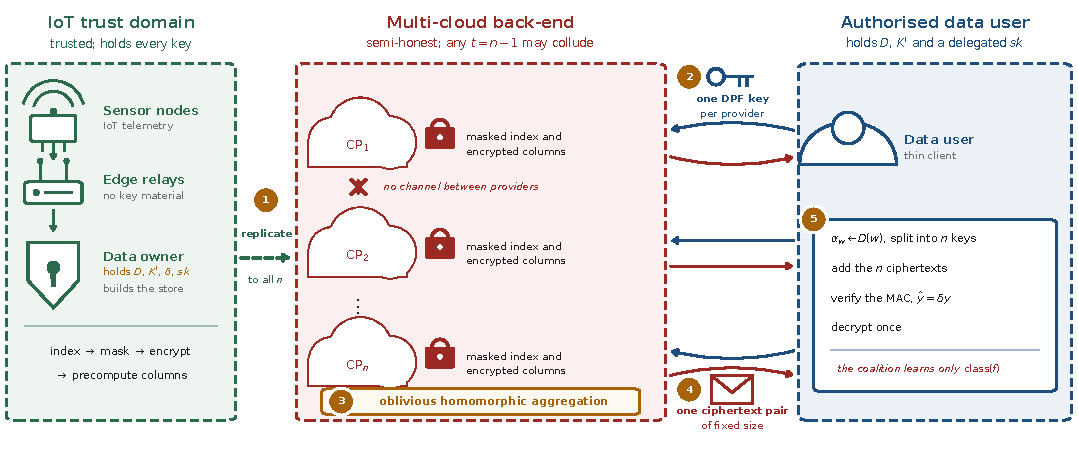
\includegraphics[width=\textwidth]{Figures/fig_architecture.pdf}
\caption{Overview of CR-SHE. The owner replicates a masked index and
encrypted columns to $n$ providers (1). A query is split into one DPF key per
provider (2), each provider aggregates obliviously over its own share (3) and
returns one ciphertext pair (4), and the user combines, verifies and decrypts
(5). No provider ever sees the matched set or its size.}
\label{fig:arch}
\end{figure*}

The workflow (Fig.~\ref{fig:arch}) has four stages. In \emph{setup}
(Algorithm~\ref{alg:outsource}), the DO derives keys, builds the pseudonymous
membership index and masks it, encrypts the computable field of every record
and its MAC counterpart, precomputes the aggregate and correction columns for
each registered template, and replicates everything to the $n$ providers. To
\emph{query}, an authorised DU looks up the keyword's row in $D$ and sends one
DPF key per provider together with the template identifier. Each provider
performs a full-domain evaluation and, without ever assembling the matched
set, returns a single ciphertext. The DU \emph{combines} the $n$ ciphertexts
and \emph{decrypts} once. Because the per-provider keys are individually
meaningless and every response is a fixed-size ciphertext, no
network-visible message depends on the queried keyword, the matched set, or
its size.

\emph{A concrete deployment.} Consider a city environmental-monitoring network
like the second corpus of Section~\ref{sec:secondcorpus}. Sensor stations
(producers) publish readings through gateways (edge relays) to the municipal
data office (DO), which replicates the encrypted, masked store to two or three
commercial clouds. Analysts at a health agency, a transport authority and a
university (DUs) run registered templates, such as the mean temperature at a
named site, the number of hours with carbon monoxide in the top decile, or a
weighted exposure score, without any cloud learning which site or condition
was asked about, or how many hours matched. Gateways only forward records over
authenticated channels; all key material stays with the DO and the analysts.

% ===========================================================================
\section{Threat model}
\label{sec:threat}

The adversary $\Adv$ is probabilistic polynomial-time, static, and
semi-honest: every corrupted party follows the protocol faithfully but pools
and analyses everything it observes. Before execution, $\Adv$ fixes a
corruption set $C\subseteq[n]$ with $|C|\le t$; the headline guarantee is
$t=n-1$, so security holds as long as at least one provider stays out of the
coalition. The defining feature is \emph{collusion}: the corrupted providers
act as a single coalition sharing state, keys, tokens and transcripts. For its
chosen $C$, the adversary observes the full static state and complete
per-query transcript of every corrupted provider,
\begin{multline*}
\mathrm{View}_C = \big( I',\ \text{CT},\ \widehat{\text{CT}},\ pk,\ pp,\\
\{A_f,\widehat{A}_f,U_f,G_f\}_f,\
\{\kappa_{q,j}\}_{j\in C,\,q\in[Q]} \big),
\end{multline*}
together with the responses those providers themselves generate. Queries are
adaptive. The security goal is that this coalition view be simulatable from
data-independent leakage revealing neither the keyword, the access pattern,
the result-set size, nor the result.

The surrounding trust assumptions are explicit. The DO and authorised DUs are
honest and hold the secret keys; data producers and in-domain edge relays hold
no secret material. All channels are authenticated and confidential, so
wiretapping yields nothing beyond what the corrupted providers already see,
and messages cannot be tampered with.

Four boundaries delimit the model. First, providers are semi-honest for the
main theorem; Section~\ref{sec:verify} adds detection of responses
inconsistent with their MAC, but full malicious security, in particular
against a provider that applies a consistent but different contraction,
requires verifiable function secret sharing and is left to future work.
Second, collusion between a data user and a provider is excluded, since an
authorised user already holds decryption capability. We do, however, treat a
client that exceeds its authority as in scope: Section~\ref{sec:auth} shows
that providers can neither restrict which rows a hidden query reads nor reject
keys for arbitrary linear combinations, which the semi-honest provider model
does not cover. Third, a single compromised DU exposes all data, because
decryption capability is delegated in full; threshold or attribute-based key
delegation is a natural extension we do not evaluate. Fourth, side channels
and traffic-volume leakage outside the message sizes accounted for here are
assumed mitigated by orthogonal system-level defences.

% ===========================================================================
\section{The CR-SHE construction}
\label{sec:construction}

\subsection{Overview}
The DO builds a membership index $I\in\{0,1\}^{N\times N_d}$ in which keyword
$w$ occupies row $\alpha_w$ and $I[\alpha_w][i]=1$ if and only if record $i$
contains $w$. Rows are assigned by a secret, append-only dictionary $D$: a
keyword receives the next free row when it first appears and keeps it for the
lifetime of the deployment, so rows never move when keywords are added
(Section~\ref{sec:ingest}). The DO shares $D$ with authorised DUs and keeps it
from the providers, because the vocabulary itself, being device and site
names, is sensitive. Which row a keyword gets carries no security weight,
since providers see neither addresses nor unmasked rows; only injectivity
matters, for correctness. Rows are fixed width, so no row is distinguishable
by size, and the index is stored masked as $I'[x][i]=I[x][i]+P[x][i]\bmod p$
with $P[x][i]=F'_{K'}(x\|i)$, an $\omega$-bit PRF output reduced modulo $p$.
The computable field of each record is encrypted as
$\text{CT}_i=\Enc_{pk}(m_i)$, with a MAC column
$\widehat{\text{CT}}_i=\Enc_{pk}(\delta m_i)$; opaque payloads are encrypted
symmetrically.

A design that first recovers the selection vector at the client and then asks
the providers to evaluate $f$ over $\{\text{CT}_i\}_{i\in S}$ destroys in the
second step exactly what the first protected, because the providers are handed
$S$. CR-SHE therefore never materialises $S$ at a provider. Each provider
contracts its own share of the selection vector against the encrypted column
and returns one ciphertext.

\subsection{Why replication rather than secret sharing}
\label{sec:whyrep}
Replication is a choice, and the obvious alternative must be answered. If the
DO instead dealt an $(n,n)$ additive sharing of each column $A_f$ over
$\mathbb{Z}_p$, every provider could answer a DPF query over its share in the
clear, giving $t=n-1$ privacy with no homomorphic encryption, no
circular-security assumption, and a response of $\lceil\log p\rceil$ bits
rather than two ciphertexts. We keep replicas for three reasons, and pay for
them in response size.

\emph{Durability.} A sharing with privacy threshold $n-1$ is lost when any one
share is lost, whereas a replica set survives the loss of $n-1$ providers,
which is the reason multi-cloud deployments replicate at all. Threshold
sharing does not escape the trade-off: a $(t{+}1,n)$ scheme tolerates
$n-t-1$ losses, so at $t=n-1$ it degenerates to the $(n,n)$ case.

\emph{Graceful degradation.} A query needs every provider in the set it is
addressed to. With replicas, queries continue over any surviving set of at
least two providers, at that set's collusion bound, without touching stored
state; a shared store cannot answer until the dealer re-shares.

\emph{Key management and churn.} Encryption under one owner key lets the owner
rotate keys, revoke a provider, or add one by copying ciphertexts. Under
sharing, every change to the provider set re-deals the whole store, and the
dealer must hold the plaintext to do it.

Table~\ref{tab:compare} lists the shared alternative as its own row. Where
durability is provided by other means and response size dominates, it is the
better design.

\subsection{Oblivious homomorphic aggregation}
\label{sec:oha}
Let $e_j[x]=\Eval(j,\kappa_j,x)$ denote provider $j$'s full-domain evaluation
vector, so that $\sum_j e_j[x]=1$ if $x=\alpha_w$ and $0$ otherwise. Provider
$j$ forms
\begin{gather*}
b_j \;=\; \sum_{x\in[N]} e_j[x]\cdot I'[x] \;\in\;\mathbb{Z}_p^{N_d},\\
\sum_{j\in[n]} b_j \;=\; b + P[\alpha_w],
\end{gather*}
where $b=I[\alpha_w]$ is the $0/1$ selection vector. It then contracts $b_j$
against the ciphertext column under the public weight vector $w_f$ of the
requested template and subtracts the mask correction described in
Section~\ref{sec:mask}:
\begin{multline*}
\text{ct}_j \;=\; \Big(\bplus_{i\in[N_d]} \big(w_f[i]\,b_j[i]\big)\bdot
\text{CT}_i\Big)\\
\bminus\; \Big(\bplus_{x\in[N]} e_j[x]\bdot U_f[x]\Big).
\end{multline*}
The DU computes $\bplus_j \text{ct}_j$ and decrypts once. Nothing that leaves
a provider depends on $b$: the response is one ciphertext of fixed size
whatever the matched set and its cardinality.

\begin{lemma}[Algebraic compatibility]
\label{lem:compat}
If the DPF output group and the HE plaintext ring are the same $\mathbb{Z}_p$,
and $\sum_{i}|w_f[i]\,m_i| < p$ for every admissible template, then for shares
$b_1,\dots,b_n\in\mathbb{Z}_p^{N_d}$ with $\sum_j b_j = \beta \bmod p$,
\begin{multline*}
\Dec_{sk}\Big(\bplus_{j\in[n]}\ \bplus_{i\in[N_d]}\ b_j[i]\bdot
\text{CT}_i\Big)\\
=\; \sum_{i\in[N_d]} \beta[i]\,m_i \pmod p .
\end{multline*}
\end{lemma}
\begin{pf}
$\bdot$ and $\bplus$ are homomorphisms over the same ring $\mathbb{Z}_p$, so
summation commutes with decryption and no reduction is lost: share addition
and plaintext addition are taken modulo the same modulus. The magnitude bound
prevents plaintext overflow. What remains is decryption correctness, which is
a noise-budget question rather than a depth question. A
plaintext-to-ciphertext product consumes no multiplicative level but scales
the noise by up to the norm of the plaintext, here as large as
$p\approx2^{36}$, because DPF shares are uniform in $\mathbb{Z}_p$, and the
contraction sums $\lceil N_d/\ell\rceil$ such products before a
rotate-and-sum. The parameters must leave room for that growth. We check the
worst case, full-magnitude coefficients across several packed chunks,
empirically rather than assume it (Section~\ref{sec:correctness}). \qed
\end{pf}

Lemma~\ref{lem:compat} is what makes the two primitives compose. Instantiating
the DPF over $\mathbb{Z}_{2^k}$ and the homomorphic scheme over an unrelated
plaintext modulus, which is the natural default since the two libraries are
chosen independently, silently breaks correctness through wraparound, and the
failure is data-dependent and therefore easy to miss in testing.

\subsection{Cancelling the index mask}
\label{sec:mask}
Because $\sum_j b_j = b + P[\alpha_w]$, the contraction above yields
$\sum_{i} w_f[i]\,b[i]\,m_i + u_f(\alpha_w)$ where the mask term is
$u_f(x)=\sum_{i} w_f[i]\,P[x][i]\,m_i$. The DO can compute $u_f(x)$ for every
$x\in[N]$ at setup, since it holds both $K'$ and the plaintext records, and
publishes the \emph{encrypted} correction column
$U_f = \big(\Enc_{pk}(u_f(x))\big)_{x\in[N]}$, packed into
$\lceil N/\ell\rceil$ ciphertexts. Providers retrieve the shared correction at
$\alpha_w$ using the \emph{same} evaluation vector $e_j$ they already
computed, so the mask is cancelled inside the ciphertext and no provider
learns either a mask value or which correction was used. The count correction
$G_f$ is this same column for a count template ($m_i\equiv1$), so it needs no
separate path; Remark~\ref{rem:whyenc} shows why it too must be encrypted.

\begin{theorem}[Index hiding]
\label{thm:mask}
Let each mask value be an $\omega$-bit output of $F'$ reduced modulo $p$. For
any two membership indexes $I_0,I_1\in\{0,1\}^{N\times N_d}$, no $\PPT$
distinguisher tells $I_0+P$ from $I_1+P$ with advantage greater than
$\advPRF_{F'}+N N_d\,2^{-\omega}$. In particular the coalition learns no
posting-list length, no keyword-frequency multiset, and no membership
relation, at a storage cost of $\lceil N/\ell\rceil$ ciphertexts per
registered template and $O(N/\ell)$ additional ciphertext operations per
provider per query.
\end{theorem}
\begin{pf}
Replace $F'$ by a truly random function at the cost of $\advPRF$. The entries
of $P$ are then independent, each distributed as $X=U\bmod p$ for $U$ uniform
on $\{0,1\}^\omega$. Writing $2^\omega=qp+r$ with $0\le r<p$, $\Pr[X=v]$ is
$(q+1)/2^\omega$ for $v<r$ and $q/2^\omega$ otherwise, so the distributions of
$X$ and $X+1\bmod p$ differ only at $v=0$ and $v=r$, by $2^{-\omega}$ at each,
and their statistical distance is at most $2^{-\omega}$. Since $I_0$ and $I_1$
differ in at most $N N_d$ entries, a hybrid over those entries gives the
bound. Costs follow by inspection of Algorithm~\ref{alg:query}. \qed
\end{pf}

The implementation reduces $\omega=64$-bit words, so for the full telemetry index
the statistical term is $N N_d\,2^{-64}\approx 2^{-31.9}$, far below anything
measurable but short of $2^{-\lambda}$. Reducing a $128$-bit block per value,
as the DPF's output conversion already does, lowers it to about $2^{-96}$ at
the cost of one extra AES call per two mask values.

\begin{remark}[Why the correction column must be encrypted]
\label{rem:whyenc}
It is tempting to publish the count correction
$g_f(x)=\sum_i w_f[i]P[x][i]$ in the clear, since it is a sum of pseudorandom
values and looks uniform. It must not be. Given $I'$ and $g_f$ in the clear,
the coalition computes $\sum_i w_f[i]I'[x][i]-g_f(x)=\sum_i w_f[i]I[x][i]$,
which for $w_f\equiv 1$ is exactly the row Hamming weight, restoring the
volume leakage the mask was introduced to remove. The correction columns $U_f$
and $G_f$ are therefore stored under HE, and the count is returned as a
ciphertext like any other aggregate.
\end{remark}

\subsection{Precomputed columns: the single-keyword fast path}
\label{sec:fast}
The contraction of Section~\ref{sec:oha} costs $\Theta(N N_d)$ ring operations
per provider per query, which is the price of hiding the access pattern
without preprocessing, by the lower bounds underlying ORAM and PIR
\citep{goldreich1996software,beimel2000reducing}. For the common case, an
aggregate over the whole posting list of a single keyword under a template
registered at setup, this cost is avoidable. The DO precomputes, for every
$x\in[N]$,
\[
A_f[x] \;=\; \sum_{i\in[N_d]} I[x][i]\,w_f[i]\,m_i \bmod p ,
\]
and publishes it as $\lceil N/\ell\rceil$ packed ciphertexts. A query then
reduces to an oblivious retrieval of one element of an encrypted length-$N$
array:
\[
\text{ct}_j \;=\; \bplus_{x\in[N]} e_j[x]\bdot A_f[x],
\]
costing $O(N)$ pseudorandom-generator calls for the full-domain evaluation
plus $O(N/\ell)$ packed ciphertext-plaintext multiplications and
$O(\log \ell)$ rotations, \emph{independent of $N_d$}. No mask correction is
needed on this path, because $A_f$ is derived from the unmasked $I$ held by
the DO and is itself encrypted.

The fast path supports the templates registered at setup, namely count, sum,
per-sensor-band sums, and fixed plaintext-weighted inner products, applied to
a single keyword. Conjunctive queries and ad-hoc weight vectors chosen at
query time fall back to the general path of Section~\ref{sec:oha}. Insertion
is cheap: a new record carrying $\tau$ tags updates $A_f$ at $\tau$ addresses
and $U_f$ at all $N$ addresses in plaintext at the DO, followed by
re-encryption of all of the column's packed ciphertexts, for the reason given
in Section~\ref{sec:ingest}; no decryption is involved.

\subsection{Verification of the aggregate}
\label{sec:verify}
Providers run the same contraction against the MAC column
$\widehat{\text{CT}}$ (or $\widehat{A}_f$ on the fast path) and return
$\widehat{\text{ct}}_j$ alongside $\text{ct}_j$. The DU decrypts both and
aborts unless $\hat{y}=\delta y$. The check is linear, and that fixes
precisely what it covers. A provider that perturbs its response by anything it
cannot also MAC, such as adding a constant, returning a stale or foreign
ciphertext, or corrupting one of the two halves, is detected except with
probability $1/p\approx2^{-36}$ over the unknown $\delta$, which is adequate
for catching faults but is not a cryptographic integrity guarantee. Two
independent MAC columns would lower this to $1/p^2\approx2^{-72}$ for one
further ciphertext per response. A provider that applies the \emph{same}
linear substitution to both halves passes: replacing its evaluation vector
$e_j$ by any $e'_j$, for instance $k\,e_j$, shifts $y$ by
$\sum_x(e'_j-e_j)[x]\,A_f[x]$ and $\hat y$ by $\delta$ times as much, so the
tag still verifies. The provider cannot aim the shift, since it knows neither
$A_f$ nor $\alpha_w$, but it can make the output wrong undetectably. The MAC
therefore protects against faulty and non-adaptive corruption, not against a
provider that deviates on purpose; Section~\ref{sec:resultsdisc} measures both
cases.

\begin{remark}[Per-row MAC keys on the fast path]
\label{rem:rowmac}
Replacing the single $\delta$ by per-row keys $\delta_x=F''_{K''}(x)$, storing
$\widehat{A}_f[x]=\delta_x A_f[x]$ and checking $\hat y=\delta_{\alpha_w}y$,
costs no additional ciphertexts or operations. A substitution $e'_j=e_j+d$
then passes only if
\[
\textstyle\sum_{x\neq\alpha_w}d[x]\,(\delta_x-\delta_{\alpha_w})\,A_f[x]=0 .
\]
For any $d$ that touches a row with $A_f[x]\neq 0$ this is a
non-zero linear form in independent uniform keys, which vanishes with
probability $1/p$. What remains undetected is a deviation concentrated on the
queried row itself, which rescales the answer; because the provider's view is
independent of $\alpha_w$, it succeeds with probability at most
$\max_x\Pr[\alpha_w=x]$, the predictability of the query. We have not
implemented or measured this variant.
\end{remark}

\subsection{Record retrieval and query authorisation}
\label{sec:auth}
When the DU needs payloads rather than an aggregate, providers return $b_j$
directly. The DU recovers $b+P[\alpha_w]$, subtracts $P[\alpha_w]$, which it
can derive locally from $K'$, and obtains $b$; no correction ciphertext is
involved. This response is $O(N_d\log p)$ bits of \emph{fixed} size,
independent of $|S|$, so the coalition learns nothing from its length. The DU
then issues a batch of $k_{\max}$ DPF-based payload retrievals padded to a
public bound, as in Splinter \citep{splinter}, so the coalition learns only
$k_{\max}$.

Authorisation interacts with obliviousness in a way that is easy to overstate.
DPF privacy hides $\alpha_w$ from every provider, so no provider can check
\emph{which} keyword a query targets: a client permitted any query can read
any row, and $N$ honest-format queries recover $I'$, hence $I$ for a client
that holds $K'$. Keys that do not encode a point function add a second
capability, that of arbitrary linear combinations of rows or of $A_f$, such as
a single aggregate over the union of many keywords, and cannot be rejected
locally either: under the $n$-party instantiation of Section~\ref{sec:prelim}
a key \emph{is} an additive share vector, so no forgery is needed, and a
well-formed two-party key is pseudorandom by the privacy property. For a fully
trusted DU, which holds $sk$ and the dictionary, none of this exceeds its
authority. It matters as soon as authority is partial, for a DU entitled to
some keywords or templates and not others, and the remedy is a proof, carried
with the key, that it encodes a point function at a permitted address, as in
PACL \citep{pacl}, or a verifiable DPF \citep{decastro2022lightweight} for
well-formedness alone. In the constructions we are aware of, including the
sketching checks of client-robust aggregation \citep{boneh2021lightweight},
the servers compare a short verification message, so adopting one relaxes
CR-SHE's no-interaction property to a single short exchange per query; whether
that exchange can be avoided is open. Our prototype checks key shape only, and
Section~\ref{sec:authresult} measures what unrestricted query access extracts.
We state per-user authorisation as a requirement rather than a solved problem.

\subsection{Dynamic ingest}
\label{sec:ingest}
IoT streams are append-only. CR-SHE keeps a static tier and a hot buffer of at
most $B$ records scanned by the same oblivious contraction; every $B$
insertions the buffer is folded into a rebuilt static tier. Because the
coalition's per-query view is independent of the query
(Theorem~\ref{thm:sec}), forward and backward privacy hold trivially: there is
no query-dependent state for an update to correlate against. Three rules keep
the update path itself from leaking.

\emph{Rows never move.} A new keyword takes the next free row of $D$. The DO
provisions $N$ above the current vocabulary, and free rows are all-zero rows
masked like any other, so a new keyword changes no public quantity; only
exhausting the headroom, which re-provisions a larger $N$, is visible.
Time-window tags make the vocabulary grow for as long as the deployment runs,
at one tag per minute on our primary corpus, so a deployment bounds $N$ by
retention, keeping one static tier per epoch (a day is $1{,}440$ minute tags)
and querying the epochs a template covers.

\emph{A fresh mask key per static tier.} A rebuild re-lays the record axis, so
reusing $K'$ would reuse mask values at new positions, and the difference of
two masked indexes would expose the change in membership. The DO therefore
draws a fresh $K'$ for every static tier, recomputes $U_f$ and $G_f$ under it,
and gives authorised DUs the current key.

\emph{Whole columns are replaced.} An insertion changes $A_f$ only at the
$\tau$ rows its tags occupy, so re-encrypting only the affected packed
ciphertexts would tell the coalition which blocks of $\ell$ rows those tags
fall in. The DO re-encrypts all $\lceil N/\ell\rceil$ ciphertexts of each
column per update batch, which is $2$ to $5$ at our corpus sizes, leaving
batch times and the public dimensions as the only dynamic leakage.

A rebuild's cost $R$ grows with the store. On the fast path it is dominated by
recomputing the precomputed columns from the postings and re-encrypting
$\lceil N/\ell\rceil$ ciphertexts per template; a deployment that also serves
the general path must rebuild and re-replicate the $\Theta(N N_d)$ masked
index. Amortisation of $R/B$ therefore holds within one tier generation, and a
long-lived deployment should merge tiers geometrically, as log-structured
stores do, to keep the amortised cost logarithmic in the store size.
Section~\ref{sec:setupresult} reports both costs.

\begin{algorithm}[t]
\footnotesize
\caption{Outsourcing at the data owner.}
\label{alg:outsource}
\begin{algorithmic}[1]
\Procedure{$\mathsf{Setup}$}{$1^\lambda,n,t,p$}
  \State $D\gets\emptyset$; \ $K'\gets\{0,1\}^\lambda$; \
         $\delta\gets\mathbb{Z}_p^{*}$
  \State $(pk,sk)\gets\mathsf{KGen}(1^\lambda,L_{\mathrm{HE}},p,\ell)$
  \State $pp\gets(n,t,N,N_d,p,\ell,\{w_f\})$
  \State \Return $(D,K',\delta,pk,sk,pp)$
\EndProcedure
\Statex
\Procedure{$\mathsf{BuildIndex}$}{$D,K',DB$}
  \State $D(w)\gets|D|$ for each new $w$
         \Comment{rows never move}
  \State $I[D(w)][i]\gets 1$ for each keyword $w$ of record $i$
  \State $I'[x][i]\gets I[x][i]+F'_{K'}(x\|i) \bmod p$
  \Statex \hfill for all $x\in[N],\,i\in[N_d]$
  \State \Return $I'$ \Comment{replicated to all $\text{CP}_j$}
\EndProcedure
\Statex
\Procedure{$\mathsf{Precompute}$}{$pk,K',DB,\{w_f\}$}
  \ForAll{registered templates $f$}
    \State $A_f[x]\gets\sum_i I[x][i]\,w_f[i]\,m_i$
    \State $\widehat{A}_f[x]\gets\delta A_f[x]$
    \State $U_f[x]\gets\sum_i F'_{K'}(x\|i)\,w_f[i]\,m_i$
    \State $G_f[x]\gets\sum_i F'_{K'}(x\|i)\,w_f[i]$
           \Comment{$U_f$, $m_i\equiv 1$}
    \State encrypt and pack each column into
    \Statex \hfill $\lceil N/\ell\rceil$ ciphertexts
  \EndFor
\EndProcedure
\Statex
\Procedure{$\mathsf{EncData}$}{$pk,DB$}
  \State $\text{CT}_i\gets\Enc_{pk}(m_i)$; \
         $\widehat{\text{CT}}_i\gets\Enc_{pk}(\delta m_i)$
  \State symmetric-encrypt opaque payloads
\EndProcedure
\end{algorithmic}
\end{algorithm}

\begin{algorithm}[t]
\footnotesize
\caption{Query, at the data user and at provider $\text{CP}_j$.}
\label{alg:query}
\begin{algorithmic}[1]
\Procedure{$\mathsf{Token}$}{$D,w,f$}
  \Comment{at the DU}
  \State $\alpha_w\gets D(w)$
  \State $(\kappa_1,\dots,\kappa_n)\gets\Gen(1^\lambda,\alpha_w,1)$
         over $\mathbb{Z}_p$
  \State \Return $(\kappa_j,f)\to\text{CP}_j$
\EndProcedure
\Statex
\Procedure{$\mathsf{FastAgg}$}{$\kappa_j,f,A_f,\widehat{A}_f$}
  \Comment{single keyword}
  \State check the shape of $\kappa_j$
         \Comment{\S\ref{sec:auth}}
  \State $e_j[x]\gets\Eval(j,\kappa_j,x)$, $x\in[N]$
         \Comment{$O(N)$ PRG}
  \State $\text{ct}_j\gets\bplus_{x} e_j[x]\bdot A_f[x]$
         \Comment{$O(N/\ell)$ HE}
  \State $\widehat{\text{ct}}_j\gets\bplus_{x} e_j[x]\bdot
         \widehat{A}_f[x]$
  \State \Return $(\text{ct}_j,\widehat{\text{ct}}_j)$
         \Comment{$O(1)$ ct}
\EndProcedure
\Statex
\Procedure{$\mathsf{GenAgg}$}{$\kappa_j,w_f,I',\text{CT},U_f$}
  \Comment{ad-hoc $w_f$}
  \State $e_j[x]\gets\Eval(j,\kappa_j,x)$, $x\in[N]$
  \State $b_j\gets\sum_{x} e_j[x]\cdot I'[x]$
         \Comment{$\Theta(N N_d)$}
  \State $\text{ct}_j\gets\bplus_i (w_f[i]b_j[i])\bdot\text{CT}_i$
  \State \hskip2em $\bminus\ \bplus_x e_j[x]\bdot U_f[x]$
  \State \Return $\text{ct}_j$ and its MAC counterpart
\EndProcedure
\Statex
\Procedure{$\mathsf{Retrieve}$}{$\kappa_j,I'$}
  \State \Return $b_j\gets\sum_{x} e_j[x]\cdot I'[x]$
         \Comment{fixed size}
\EndProcedure
\Statex
\Procedure{$\mathsf{CombineDec}$}{$sk,K',\delta,\cdot$}
  \Comment{at the DU}
  \State $y\gets\Dec(sk,\bplus_j\text{ct}_j)$
  \State $\hat{y}\gets\Dec(sk,\bplus_j\widehat{\text{ct}}_j)$
  \State \textbf{abort} if $\hat{y}\neq\delta y$
         \Comment{missed w.p.\ $1/p$}
  \State retrieval: $b\gets(\sum_j b_j)-P[\alpha_w]$
  \State \hskip2em $S\gets\{i: b[i]=1\}$
  \State \Return $y$, and $S$ if retrieving
\EndProcedure
\end{algorithmic}
\end{algorithm}

\subsection{Worked instance}
A clinician queries the tag \texttt{arrhythmia} with the registered template
\textsc{mean}. The DU derives $\alpha_w$ and sends one DPF key per provider.
Each provider performs a full-domain pass, contracts against the packed
\textsc{sum} and \textsc{count} columns, and returns two ciphertexts plus
their MAC counterparts. The DU adds the shares, verifies the MACs, decrypts,
and divides. No provider, and no coalition of up to $n-1$, learns the tag
queried, which records contributed, how many did, or the mean itself.

% ===========================================================================
\section{Security analysis}
\label{sec:security}

\emph{Leakage profile.} We define
$\Leak=(\Leak_{\mathrm{Setup}},\Leak^{\text{CP}},\Leak^{\text{DU}})$ with an
observer split:
\begin{align*}
\Leak_{\mathrm{Setup}}(DB) &= (n,t,N,N_d,p,\ell,\{w_f\}),\\
\Leak^{\text{CP}}_{\mathrm{Query}} &= \mathrm{class}(f),\\
\Leak^{\text{DU}}_{\mathrm{Query}} &= \big(|S|,\ f(\mathrm{records}(S))\big).
\end{align*}
The coalition learns which registered template was requested and the public
dimensions of the deployment, and nothing else: not the keyword, not the
access pattern, not $|S|$, not the result. In contrast to a design in which
the matched set is returned to the providers for evaluation, and in contrast
to an unmasked index, $\Leak_{\mathrm{Setup}}$ here contains no posting-list
lengths and no membership structure, by Theorem~\ref{thm:mask}. Retrieval adds
the public padding bound $k_{\max}$ to $\Leak^{\text{CP}}$. A conjunctive
query is two selections intersected at the DU, adding only result sizes to
$\Leak^{\text{DU}}$, never to the coalition.

\begin{definition}[$\Leak$-security against $t$-collusion]
\label{def:sec}
In $\Real_{\Adv,\Pi}(1^\lambda)$: (1) $\Adv$ outputs $(DB,C)$ with $|C|\le t$;
(2) the challenger runs $\mathsf{Setup}$, $\mathsf{BuildIndex}$,
$\mathsf{Precompute}$, $\mathsf{EncData}$ and gives $\Adv$ the static view
$(I',\text{CT},\widehat{\text{CT}},\{A_f,\widehat A_f,U_f,G_f\}_f,pk,pp)$;
(3) for $q=1,\dots,Q$, $\Adv$ adaptively issues a keyword $w_q$ with template
$f_q$ and receives the coalition's per-query view
$\big(\{\kappa_{q,j}\}_{j\in C},\{\text{ct}_{q,j}\}_{j\in C}\big)$; (4) $\Adv$
outputs a bit. In $\Ideal_{\Adv,\Sim,\Leak}(1^\lambda)$ a $\PPT$ simulator
$\Sim$ produces the views given only $\Leak_{\mathrm{Setup}}$ and the
per-query leakage. $\Pi$ is $\Leak$-adaptively-secure against $t$-collusion if
for every $\PPT$ $\Adv$ corrupting $\le t$ providers there is a $\PPT$ $\Sim$
with $|\Pr[\Real=1]-\Pr[\Ideal=1]|\le\negl(\lambda)$.
\end{definition}

\begin{theorem}[Correctness]
\label{thm:correct}
Fix a database $DB$, a keyword $w$, and a registered template $f$ satisfying
the magnitude bound of Lemma~\ref{lem:compat}. Then $\mathsf{CombineDec}$
returns $y=\sum_{i\in S} w_f[i]\,m_i$ with $S=\{i: I[\alpha_w][i]=1\}$ on both
the fast and general paths, and $\mathsf{Retrieve}$ returns exactly $S$,
except with the negligible probability that leveled-HE decryption fails.
\end{theorem}
\begin{pf}
By DPF correctness $\sum_j e_j[x]=1$ at $x=\alpha_w$ and $0$ elsewhere.

\emph{Fast path.} $\bplus_j\text{ct}_j$ decrypts, by Lemma~\ref{lem:compat}
applied with $\beta=\big(\sum_j e_j\big)$ over the array $A_f$, to
$A_f[\alpha_w]=\sum_i I[\alpha_w][i]w_f[i]m_i=\sum_{i\in S}w_f[i]m_i$.

\emph{General path.} $\sum_j b_j=\sum_x\big(\sum_j e_j[x]\big)
I'[x]=I'[\alpha_w]=b+P[\alpha_w]$. By Lemma~\ref{lem:compat} the first term of
$\bplus_j \text{ct}_j$ decrypts to $\sum_i w_f[i](b[i]+P[\alpha_w][i])m_i$ and
the second to $u_f(\alpha_w)=\sum_i w_f[i]P[\alpha_w][i]m_i$; their difference
is $\sum_{i\in S}w_f[i]m_i$.

\emph{Retrieval.} $\big(\sum_j b_j\big)-P[\alpha_w]=b$ exactly, and the DU
derives $P[\alpha_w]$ from $K'$.

The dictionary is injective by construction, so row $\alpha_w$ is exactly the
records containing $w$. Decryption correctness under the noise growth
discussed in the proof of Lemma~\ref{lem:compat} contributes the negligible
failure term. The MAC check passes with certainty for honest providers, since
$\delta$ distributes over the linear contraction. \qed
\end{pf}

\begin{theorem}[$t$-collusion leakage security]
\label{thm:sec}
If $F'$ is a secure PRF, $(\Gen,\Eval)$ is an $(n{-}1)$-private DPF, and the
homomorphic and symmetric schemes are IND-CPA, then CR-SHE is
$\Leak$-adaptively-secure against $t$-collusion in the sense of
Definition~\ref{def:sec}, for $t=n-1$ and
$\Leak^{\text{CP}}_{\mathrm{Query}}=\mathrm{class}(f)$. Concretely, for every
$\PPT$ $\Adv$ there exist $\PPT$ $\Sim$ and $B_1,\dots,B_3$ with
\begin{multline*}
\big|\Pr[\Real{=}1]-\Pr[\Ideal{=}1]\big|\\
\le\ \mathrm{Adv}^{\mathrm{PRF}}_{B_1} + N N_d\,2^{-\omega}\\
+\ Q\cdot\mathrm{Adv}^{\mathrm{DPF}}_{B_2}
+\ m\cdot\mathrm{Adv}^{\mathrm{CPA}}_{B_3},
\end{multline*}
where $m$ is the number of ciphertexts in the coalition view. As is standard
for BFV, IND-CPA is assumed to hold even given the relinearisation and
rotation keys the providers need (circular security). The theorem is stated
for one static tier; with a fresh $K'$ per tier
(Section~\ref{sec:ingest}) it applies to each tier independently, with one PRF
term per tier.
\end{theorem}
\begin{pf}
Take $|C|=n-1$ without loss of generality; a smaller coalition holds a subset
of the same state. Let $H_0=\Real$.

\emph{$H_1$ (PRF to random, index to zero).} Replace $F'$ by a truly random
function, at cost $\mathrm{Adv}^{\mathrm{PRF}}_{B_1}$. Then build $I'$ from
the all-zero index instead of $I$, which by the statistical step of
Theorem~\ref{thm:mask} costs at most $N N_d\,2^{-\omega}$; $I'$ now depends
only on $(N,N_d)$.

\emph{$H_2$ (DPF keys to simulated).} Replace $\{\kappa_{q,j}\}_{j\in C}$ by
$\Sim_{\mathrm{DPF}}(1^\lambda,C,N)$, licensed by $(n{-}1)$-privacy; a hybrid
over the $Q$ queries costs $Q\cdot\mathrm{Adv}^{\mathrm{DPF}}_{B_2}$. The
per-query key material now depends only on $(C,N)$.

\emph{$H_3$ (ciphertexts to encryptions of $0$).} Replace each of the $m$
ciphertexts in the coalition view, namely $\text{CT}$, $\widehat{\text{CT}}$
and the columns $A_f,\widehat A_f,U_f,G_f$, by encryptions of $0$ under $pk$,
at cost $m\cdot\mathrm{Adv}^{\mathrm{CPA}}_{B_3}$, since the coalition holds
only $pk$.

\emph{Simulator.} The responses $\text{ct}_{q,j}$ need not be simulated
separately: each is a deterministic function of $\kappa_{q,j}$, the template
identifier, and the provider's stored state, all of which $\Sim$ possesses in
$H_3$. $\Sim$ therefore regenerates the entire coalition view from
$\Leak_{\mathrm{Setup}}$ and $\mathrm{class}(f)$ alone, so
$\Ideal_{\Adv,\Sim,\Leak}$ matches $H_3$; summing the four terms proves the
theorem. \qed
\end{pf}

\begin{remark}[Why the two-round design admits no such bound]
\label{rem:v1}
Suppose the client recovers $S$ and then requests
$\Compute(pk,\{\text{CT}_i\}_{i\in S},f)$ from the providers. The coalition's
per-query view then contains $S$ itself, which is a function of the queried
keyword and the database. No simulator given only data-independent leakage can
produce it, so an empty per-query leakage profile is \emph{unattainable} in
that design rather than merely loose. Contracting at the provider is what
makes Theorem~\ref{thm:sec} true as stated.
\end{remark}

\begin{remark}[Content confidentiality and graceful degradation]
For two databases of equal public dimensions differing only in contents,
Theorem~\ref{thm:sec} makes each coalition view indistinguishable from a
distribution depending only on $\Leak_{\mathrm{Setup}}$, which is identical
for both; the executions differ by at most $m\cdot\mathrm{Adv}^{\mathrm{CPA}}$,
with the content dependence isolated in $H_3$. The same proof applies for any
$|C|\le n-1$, since $(n{-}1)$-privacy holds for every strict subset; a
coalition of all $n$ providers is outside the model, and against it the
guarantee degrades to IND-CPA confidentiality of the records with the index
still masked under $F'$.
\end{remark}

\begin{remark}[Beyond semi-honest]
Section~\ref{sec:verify} detects a response inconsistent with its MAC except
with probability $1/p$. It does not detect a provider that applies the same
linear substitution to both halves, that is, a contraction against any vector
other than its evaluation share, nor does it guarantee output delivery. Full
malicious security through verifiable function secret sharing remains future
work, which is why Table~\ref{tab:compare} records \emph{detect} rather than
$\checkmark$.
\end{remark}

% ===========================================================================
\section{Complexity analysis}
\label{sec:complexity}

Table~\ref{tab:complexity} summarises the asymptotic costs. Three entries
deserve comment because they correct the intuitive accounting.

First, the selection contraction on the general path is $\Theta(N N_d)$ ring
operations, not $\Theta(N)$: a full-domain evaluation produces $N$ share
values, each of which multiplies an index \emph{row} of width $N_d$. Counting
only the $O(N)$ pseudorandom-generator calls of the evaluation omits the
dominant term. With a small modulus and vectorised arithmetic these are cheap
word operations, and the pass is embarrassingly parallel, but the asymptotic
is what it is: this is the ORAM and PIR lower-bound price for hiding the
access pattern from a coalition without preprocessing
\citep{goldreich1996software,beimel2000reducing}; preprocessing PIR avoids it
at the cost of client hints that updates invalidate
\citep{corrigan2020private}.

Second, the fast path of Section~\ref{sec:fast} removes the $N_d$ factor
entirely, at $O(N)$ generator calls plus $O(N/\ell)$ packed ciphertext
operations, at the cost of restricting queries to single keywords and
templates registered at setup.

Third, the aggregate response is $O(1)$ ciphertexts and, crucially,
\emph{independent of $|S|$}. A response whose size grew with the result set
would leak the result-set size to the coalition and contradict
$\Leak^{\text{CP}}$. Retrieval responses are $O(N_d\log p)$ bits of fixed size
for the same reason.

\begin{table}[pos=t]
\caption{Asymptotic costs. $\gamma$ is the per-provider DPF key size,
$O(\lambda\log N)$ at $n=2$; $\ell$ is the SIMD slot count.}
\label{tab:complexity}
\centering
\scriptsize
\setlength{\tabcolsep}{2pt}
\renewcommand{\arraystretch}{1.2}
\begin{tabular*}{\tblwidth}{@{\extracolsep{\fill}}lll@{}}
\toprule
Resource & Per provider & Data user \\
\midrule
Index storage           & $O(N N_d\log p)$                  & n/a \\
Ciphertext storage      & $O(N_d)+O(N/\ell)$ per $f$        & n/a \\
Query uplink            & $O(\gamma)$                       & $O(n\gamma)$ \\
Aggregate downlink      & $O(1)$ ct                         & $O(n)$ ct \\
Retrieval downlink      & $O(N_d\log p)$, fixed             & $O(nN_d\log p)$ \\
Selection, fast         & $O(N)$ PRG, $O(N/\ell)$ HE        & 1 decrypt \\
Selection, general      & $O(N)$ PRG, $\Theta(NN_d)$ ring   & 1 decrypt \\
Aggregate HE ops        & $O(N_d/\ell)$ or $O(N/\ell)$      & $O(n)$ adds \\
Owner precomputation    & $O(NN_d)$ per $f$ per tier        & n/a \\
Insertion, $\tau$ tags  & $O(N)$ plaintext updates          & n/a \\
\bottomrule
\end{tabular*}
\end{table}

% ===========================================================================
\section{Implementation}
\label{sec:impl}

We implement CR-SHE end to end in C++17, together with the corpus builder
and one benchmark script per figure.

\emph{Distributed point function.} The two-party DPF is the
Boyle-Gilboa-Ishai GGM-tree construction with a fixed-key AES-128
pseudorandom generator in the Matyas-Meyer-Oseas form
$G(s)=\mathrm{AES}_k(s)\oplus s$ under three independent fixed keys, giving
two child seeds and one conversion block per node. Three code paths are
provided, for x86-64 AES-NI, ARMv8 crypto extensions, and a portable
software fallback, and every binary reports at start-up which one it took; the
measurements below were taken with AES-NI. Full-domain evaluation traverses
the tree once, processing nodes in pairs so that four independent AES chains
are in flight, and converts leaves four at a time. The implementation is
verified exhaustively against the point function at every point of the domain
for depths up to $12$ and for $n\in\{2,3,4,5\}$.

\emph{Homomorphic layer.} Leveled BFV through OpenFHE~1.2.3
\citep{openfhe}, at plaintext modulus $p=68{,}724{,}326{,}401$, a $37$-bit
prime with $p\equiv 1 \bmod 2^{17}$ so that batching is available at every
ring dimension up to $65{,}536$, ring dimension $8{,}192$, $\ell=8{,}192$ SIMD
slots, multiplicative depth $1$, at the $128$-bit classical security level.
The one contraction is a plaintext-to-ciphertext product followed by a
rotate-and-sum over the batch.

\emph{Lemma~\ref{lem:compat} as a type, not a comment.} The DPF output group
and the BFV plaintext ring are the same object in the code: a single modulus
type is constructed once and consumed by the DPF, the index mask, and the
homomorphic backend. The failure mode the lemma warns about, a DPF over
$\mathbb{Z}_{2^k}$ composed with an unrelated plaintext modulus, is therefore
unrepresentable rather than merely documented. The magnitude bound is checked
against the corpus at setup, and a corpus that would violate it is rejected
rather than silently wrapped.

\emph{Selection arithmetic.} The general-path contraction accumulates in $128$
bits and reduces once per output: each product is below $p^2<2^{74}$ and at
most $N\le 2^{16}$ of them are summed on either corpus, so the accumulator
cannot overflow and the inner loop is a single multiply-add. The pass is
parallelised over tag blocks with per-thread accumulators.

\emph{Deployment.} The implementation separates a deployment bundle along
the trust boundary: the public half carries the crypto context, the evaluation keys,
$pk$ and the precomputed columns, and the provider process loaded from it
holds no secret key and refuses decryption. We exercise this with
$n\in\{2,3,4\}$ independent provider processes and a client communicating over
TCP. We report it as a \emph{single-host} deployment
(Section~\ref{sec:wanresult}): the processes are genuinely separate and the
protocol is the real one, but they run on one machine over the loopback
interface, so the transport component is framing and serialisation only and
excludes wide-area latency. Section~\ref{sec:limits} returns to what this
omits.

\emph{Randomness and keys.} Every secret the protocol samples, from DPF root
seeds to the seeds of the $n$-party construction and the owner's $K'$ and
$\delta$, is drawn from the operating system's CSPRNG, never from a seeded
generator. The benchmark harness is the one exception: it derives the owner's
keys from a fixed public seed so that the leakage experiment and the
correctness tests reproduce bit for bit, and such keys are never used in a
deployment bundle. Mask values are $\omega=64$-bit AES-CTR words reduced
modulo $p$ (Theorem~\ref{thm:mask}). The dictionary assigns rows in
sorted tag-name order when a corpus is built; it does not implement the
insertion of new keywords or the per-tier re-keying of
Section~\ref{sec:ingest}, which the static benchmarks below do not exercise.

\emph{Corpora.} The primary corpus is the Environmental Sensor Telemetry
dataset of $405{,}184$ MQTT messages from three Raspberry-Pi sensor arrays,
each carrying a device identifier, a timestamp, and readings for carbon
monoxide, humidity, liquid petroleum gas, smoke, temperature, light and motion
\citep{stafford_2020_environmental}. Records are indexed under the metadata
tags a deployed IoT platform would attach: the device identifier, a one-minute
time window, decile bands of each of the five continuous sensor channels, and
the two boolean flags. This yields $N=11{,}580$ tags over $3{,}646{,}656$
postings, with heavy-tailed posting lists of median $35$, mean $314.9$ and
maximum $404{,}702$ (Fig.~\ref{fig:postcdf}). Aggregation operates on the real
temperature readings, scaled to hundredths of a degree, so one coherent
dataset drives both retrieval and analytics. The largest admissible single-tag
aggregate is $908{,}575{,}470$, leaving $75.6\times$ headroom below $p$.

That corpus has only three physical devices, so the whole evaluation is
repeated on a second one, the UCI Beijing Multi-Site Air-Quality dataset of
$420{,}768$ hourly records from \emph{twelve} monitoring sites over four years
\citep{zhang2017cautionary}, which triples the tag domain and supplies the
device diversity the first corpus lacks. Section~\ref{sec:secondcorpus}
reports it in full; both corpora are built by the same script, from the
published raw files, with no hand curation.

\emph{Baselines.} We compare against (i) a plaintext linear scan; (ii) a
single-server searchable-encryption scheme with PRF tokens and AES-CTR posting
lists, which leaks the search pattern, the access pattern and $|S|$; (iii)
non-recursive Path ORAM with bucket size $Z=4$ and a client-side position map,
charging one access per matched record plus one for the index entry; (iv) a
distributed-trust, search-only baseline in the style of DORY \citep{dory},
which is our own selection path stopped at the selection vector and therefore
isolates exactly the cost of adding oblivious analytics to oblivious
selection; and (v) a \emph{faithful} homomorphic equality scan, which pays the
cost of a homomorphic equality per record,
$\mathrm{eq}(a,b)=1-(a-b)^{q-1}$ by Fermat over a plaintext prime $q$, at the
multiplicative depth that implies; a cheaper proxy that charged one
homomorphic addition per item would understate this alternative by orders of
magnitude. For (v) one full batch of $\ell$ slots is measured and the corpus
total is obtained by multiplying by the batch count; both the measured batch
cost and the extrapolation factor are reported, and extrapolated quantities
are marked as such throughout.

\emph{Hardware.} All measurements were taken on one AMD EPYC~7J13 machine with
$64$ cores and $64$\,GB of RAM running Ubuntu~24.04, with AES-NI, GCC~13 and
OpenMP. Latencies are medians of $11$ runs unless stated otherwise, with the
interquartile range recorded per run and drawn as error bars in the
figures. Every binary prints the CPU, thread count, AES backend and
homomorphic parameters it ran under, and every results row repeats them, so no
number in this section can be separated from the machine that produced it.

\emph{What a fast-path latency includes.} The protocol always computes both
contractions, value and MAC, so every fast-path figure includes the MAC and
every aggregate response is two ciphertexts; we did not measure a MAC-free
variant. The fast-path figures differ in two respects only: whether the timed
region includes the provider's full-domain DPF evaluation, and how many
threads that evaluation uses, which matters because its OpenMP team competes
with OpenFHE's own thread pool. With the evaluation on all $64$ threads
(Tables~\ref{tab:compute}, \ref{tab:baselines} and~\ref{tab:beijing}) a query
costs $38.8$--$41.2$\,ms across the two corpora; with it on one thread, as the
deployed provider runs it, $34.3$--$35.5$\,ms on the primary corpus
(Section~\ref{sec:scaling}, Table~\ref{tab:wan}); and the two contractions
alone, without the evaluation, $33.6$\,ms. Serialisation is excluded
everywhere except the transport column of Table~\ref{tab:wan}.

% ===========================================================================
\section{Results analysis and discussion}
\label{sec:resultsdisc}

\subsection{Correctness}
\label{sec:correctness}
Every measurement below is taken against an implementation that first has to
compute the right answer, so we report that check first. On a
$5{,}000$-record subsample of the primary corpus, for $n\in\{2,3,4\}$ and all
four registered templates, the decrypted aggregate equals the plaintext ground
truth exactly and the MAC verifies for $1{,}000$ randomly drawn tags per
template on the fast path and $50$ on the general path; retrieval returns
exactly the posting list; and the aggregate downlink is byte-identical for
matched sets of size $0$ and $4{,}999$. The homomorphic test suite separately
multiplies full-magnitude $\mathbb{Z}_p$ coefficients across several packed
chunks, the general path's worst case for noise. The same battery passes
unchanged when the same build is repeated on a second, $16$-core host. This is Theorem~\ref{thm:correct} in practice, including the mask
cancellation of Section~\ref{sec:mask}, which is the step most likely to fail
silently. Section~\ref{sec:secondcorpus} repeats the same battery on the
second corpus.

\subsection{Selection latency and key size}
Table~\ref{tab:search} and Fig.~\ref{fig:searchlat} report the per-provider
full-domain evaluation, which is the whole of the selection phase. Selection
depends on the tag domain alone, so one table covers both corpora. At the
primary corpus's $N=11{,}580$ it costs $0.336$\,ms on one thread and
$0.177$\,ms at sixteen; at $N=10^6$ it costs $45.7$\,ms on one thread and
$18.8$\,ms at thirty-two. The two-party key is $266$\,B at that domain,
growing to $368$\,B at $N=10^6$, consistent with the $O(\lambda\log N)$ bound.

Selection does not scale past about sixteen to thirty-two threads and then
regresses: at $N=11{,}580$ it improves from $0.336$\,ms to $0.177$\,ms at
sixteen threads but returns to $0.211$\,ms at sixty-four, and at $N=10^6$ from
$45.7$\,ms to $18.8$\,ms at thirty-two and back to $24.4$\,ms at sixty-four.
The per-level work at these domain sizes is too small to amortise thread
dispatch across all cores of a $64$-core part. A deployment should pin the
selection pass to the knee.

These are sub-millisecond quantities on a shared cloud host, and they carry
correspondingly loose error bars: repeated runs of the identical binary differ
by up to $25\%$ at $N\approx10^4$, while the $N=10^6$ figures, where each
measurement is tens of milliseconds, repeat to within $1\%$. The table gives
medians of $21$ runs, and the interquartile range is recorded for every
cell. Conclusions in this subsection are drawn only at the
order-of-magnitude level, which is robust to that variation; the like-for-like
comparison that matters is made in Section~\ref{sec:aggresult}, where the
quantities are tens of milliseconds.

Set against the homomorphic half of the same query, the scale is what matters:
selection is under $0.2$\,ms while the packed contraction that follows it is
tens of milliseconds (Section~\ref{sec:aggresult}). The symmetric-key half of
CR-SHE is not the bottleneck, which is the design's intent: symmetric work on
the selection path, homomorphic operations only on the aggregate.

\begin{table}[pos=t]
\caption{Per-provider selection latency and two-party key size against $N$.
Medians of 21 runs.}
\label{tab:search}
\centering
\footnotesize
\setlength{\tabcolsep}{2pt}
\renewcommand{\arraystretch}{1.2}
\begin{tabular*}{\tblwidth}{@{\extracolsep{\fill}}lcccccc@{}}
\toprule
$N$ & \multicolumn{5}{c}{Latency (ms), $T$ threads} & Key \\
\cmidrule(lr){2-6}
    & $T=1$ & $4$ & $16$ & $32$ & $64$ & (B) \\
\midrule
$1{,}000$    & $0.032$  & $0.032$  & $0.032$  & $0.032$  & $0.032$  & $198$ \\
$10{,}000$   & $0.290$  & $0.175$  & $0.156$  & $0.161$  & $0.183$  & $266$ \\
$11{,}580$   & $0.336$  & $0.200$  & $0.177$  & $0.181$  & $0.211$  & $266$ \\
$100{,}000$  & $4.418$  & $2.487$  & $1.909$  & $1.928$  & $2.420$  & $317$ \\
$10^{6}$     & $45.741$ & $25.701$ & $19.711$ & $18.769$ & $24.401$ & $368$ \\
\bottomrule
\end{tabular*}
\end{table}

\subsection{Oblivious aggregation}
\label{sec:aggresult}
This is the central claim of the paper, and Table~\ref{tab:compute} and
Fig.~\ref{fig:complat} test it directly.

On the fast path the provider's aggregate latency is $38.8$--$39.2$\,ms across
a $405\times$ range of record counts, from $N_d=10^3$ to the full
$N_d=405{,}184$, a spread of $\pm0.5\%$, that is, flat. An initial sweep taken
in increasing $N_d$ showed the first four points near $53$\,ms and the last
four near $38.5$\,ms; because that step is \emph{anti}-correlated with $N_d$,
we repeated the sweep in decreasing order, which reproduced
$38.8$--$39.2$\,ms at every point including $N_d=10^3$. The step was therefore
a warm-up artefact of run ordering and not a dependence on $N_d$, and
Table~\ref{tab:compute} quotes the order-controlled run.

On the general path the same aggregate costs $103.7$\,ms at $N_d=10^3$ and
$1{,}378.2$\,ms at the full corpus, which is $35.5\times$ the fast path. The
growth is mild up to $N_d\approx5\times10^4$, where the fixed homomorphic cost
still dominates, and then tracks the $\Theta(N N_d)$ contraction, giving
$196.8$, $539.5$ and $1{,}378.2$\,ms at $10^5$, $2\times10^5$ and
$4.05\times10^5$: a factor of $2.74$ for the doubling and $2.55$ for the
$2.03\times$ step that follows. The slight superlinearity is memory
bandwidth: at full scale the masked index is $37.5$\,GB and every query
streams all of it.

That storage is the general path's real constraint. The masked index is
$N\times N_d$ elements of $\mathbb{Z}_p$, which is $9.26$\,GB at $N_d=10^5$
and $37.5$\,GB at the full corpus, \emph{per provider} and replicated $n$
times. It fits on a $64$\,GB machine and not on a smaller one, and it must be
resident for every query. This is the price of a fully general oblivious
selection and it is the reason the fast path exists.

Per-query downlink is $525{,}950$\,B per provider, being two ciphertexts, the
aggregate and its MAC, and is byte-identical for every $N_d$ and, more
importantly, for every $|S|$. We verify this directly by querying a tag whose
posting list is empty and one that matches $4{,}999$ of the $5{,}000$ records
in the test subsample, and comparing the serialised responses byte for byte. A
design that returned the selection vector instead would send $O(N_d\log p)$
bits, $800{,}000$\,B at $N_d=10^5$, and would leak $|S|$ through the response
size itself.

\begin{table}[pos=t]
\caption{Aggregate latency and storage, fast against general path,
$N=11{,}580$, template \textsc{sum}. Medians of $11$ runs (fast) and $3$
(general).}
\label{tab:compute}
\centering
\footnotesize
\setlength{\tabcolsep}{3pt}
\renewcommand{\arraystretch}{1.2}
\begin{tabular*}{\tblwidth}{@{\extracolsep{\fill}}lcccc@{}}
\toprule
$N_d$ & Fast & General & $I'$ / provider & Downlink \\
      & (ms) & (ms)     & (GB)            & (B) \\
\midrule
$10^3$             & $38.8$ & $103.7$   & $0.09$  & $525{,}950$ \\
$5\times10^3$      & $39.0$ & $106.9$   & $0.46$  & $525{,}950$ \\
$10^4$             & $38.8$ & $111.9$   & $0.93$  & $525{,}950$ \\
$2\times10^4$      & $38.8$ & $121.7$   & $1.85$  & $525{,}950$ \\
$5\times10^4$      & $39.1$ & $120.7$   & $4.63$  & $525{,}950$ \\
$10^5$             & $39.2$ & $196.8$   & $9.26$  & $525{,}950$ \\
$2\times10^5$      & $39.1$ & $539.5$   & $18.53$ & $525{,}950$ \\
$4.05\times10^5$   & $38.8$ & $1{,}378.2$ & $37.54$ & $525{,}950$ \\
\bottomrule
\end{tabular*}
\end{table}

\subsection{Comparison against baselines}
Table~\ref{tab:baselines} places CR-SHE against the five baselines on the
primary corpus, the same machine and the same probe tag, whose posting list
has that corpus's median length $|S|=35$.

The ordering is the expected one and the magnitudes are the point. A plaintext
scan is free and private against nobody. Single-server searchable encryption
is also essentially free and leaks the search pattern, the access pattern and
$|S|$; its downlink grows with the result set. Path ORAM hides the access
pattern from one server at $1.6\,\mu$s per access, but pays per matched
record, so its cost and its $373$\,kB downlink both scale with $|S|$ while
CR-SHE's do not. The DORY-style distributed-trust baseline, our own selection
path stopped at the selection vector, costs $130.4$\,ms, and two comparisons
against it answer different questions. Like for like, the general path
computes the same selection and then aggregates obliviously over it in
$196.8$\,ms at the same $N_d$ (Table~\ref{tab:compute}): oblivious analytics
adds about half again to oblivious selection, not an order of magnitude. The
fast path answers the narrower question of a registered single-keyword
aggregate in $39.2$\,ms, which is $3.3\times$ \emph{less} than materialising
the selection vector, because it never touches the $N\times N_d$ index; that
gain is bought by restricting the query class, not by a cheaper selection.

The faithful homomorphic equality scan is the comparison that depends most on
charging the right operation. At $q=65{,}537$ a single digit suffices for the
tag domain, but the Fermat exponentiation needs $16$ squarings, plus one level
for the product with the record value: multiplicative depth $17$, and ring
dimension $32{,}768$. One batch of $32{,}768$ slots costs $1.86$\,s and the
corpus needs $13$ batches, giving $24.2$\,s per query, extrapolated, which is
$617\times$ the CR-SHE fast path. Charging one homomorphic addition per item
instead would place this baseline in the tens of milliseconds and invert the
conclusion.

\begin{table}[pos=t]
\caption{Baselines, same corpus and machine, $N_d=10^5$, probe tag with the
median $|S|=35$. $\dagger$ marks an extrapolated value.}
\label{tab:baselines}
\centering
\footnotesize
\setlength{\tabcolsep}{3pt}
\renewcommand{\arraystretch}{1.2}
\begin{tabular}{@{}lcc>{\raggedright\arraybackslash}p{2.1cm}@{}}
\toprule
System & Server & Downlink & Leakage to the \\
       & (ms)   & (B)      & server(s) \\
\midrule
Plaintext scan        & $<0.001$ & $8$              & everything \\
SSE, 1 server         & $<0.001$ & $560$            & search and access
pattern, $|S|$ \\
Path ORAM             & $0.059^{\dagger}$ & $373{,}248$ & $|S|$, via access
count \\
DORY-style search     & $130.4$  & $800{,}000$      & none; no analytics \\
FHE equality scan     & $24{,}157^{\dagger}$ & n/a & none; 1 server \\
\midrule
\textbf{CR-SHE, fast} & $\mathbf{39.2}$ & $\mathbf{525{,}950}$ &
$\mathrm{class}(f)$ only \\
\bottomrule
\end{tabular}
\end{table}

\subsection{Multi-cloud deployment}
\label{sec:wanresult}
We ran the full protocol between independent provider processes and a client,
in the deployment split described in Section~\ref{sec:impl}, for
$n\in\{2,3,4\}$, $100$ queries each.

\emph{Provider compute is flat in $n$} (Table~\ref{tab:wan}): $34.82$, $34.85$
and $35.48$\,ms for $n=2,3,4$. This is the measurement that supports the
central structural claim about cost, namely that the client waits on the
slowest provider and not on their sum. End-to-end latency rises only from
$44.1$\,ms to $52.5$\,ms across the same range, and the increase is transport,
at $8.3$, $9.1$ and $15.5$\,ms, because the client receives $n$ responses of
$525{,}950$\,B each and deserialises them. Client-side combine, MAC
verification and decryption cost $1.37$--$1.63$\,ms and are essentially
independent of everything else, which is what makes the design viable for a
thin data user.

The caveat is the one stated in Section~\ref{sec:impl}: all providers ran on
one machine over loopback, so the transport figure is framing, serialisation
and the loopback stack, and contains no wide-area latency. A real deployment
adds the inter-region round-trip to the transport component and leaves
provider compute and client cost unchanged. We do not extrapolate a wide-area
number from this measurement.

\begin{table}[pos=t]
\caption{Single-host deployment over loopback, medians of 100 queries.
Transport excludes wide-area latency.}
\label{tab:wan}
\centering
\footnotesize
\setlength{\tabcolsep}{3pt}
\renewcommand{\arraystretch}{1.2}
\begin{tabular*}{\tblwidth}{@{\extracolsep{\fill}}lcccc@{}}
\toprule
$n$ & End-to-end & Provider & Transport & Client \\
    & (ms)       & (ms)     & (ms)      & (ms) \\
\midrule
$2$ & $44.12$ & $34.82$ & $8.30$  & $1.37$ \\
$3$ & $45.40$ & $34.85$ & $9.09$  & $1.52$ \\
$4$ & $52.53$ & $35.48$ & $15.48$ & $1.63$ \\
\bottomrule
\end{tabular*}
\end{table}

\subsection{Communication}
\label{sec:commresult}
At $N=11{,}580$ the two-party construction sends a $266$\,B key to each
provider, $532$\,B of uplink in total. The non-succinct $n$-party
instantiation used for $n>2$ sends $32$\,B to each of $n-1$ providers and
$92{,}656$\,B to one, so total uplink is $92{,}688$\,B at $n=2$,
$92{,}720$\,B at $n=3$ and $92{,}752$\,B at $n=4$. Tolerating more collusion
is therefore nearly free in this instantiation, but moving beyond two
providers at all costs a factor of $174$ in uplink over the succinct two-party
tree. Fig.~\ref{fig:comm} plots both against $N$. A succinct
$(n{-}1)$-private instantiation would reduce the heavy key from $O(N\log p)$
to $O(2^{n/2}\sqrt{N}\lambda)$.

Downlink is $525{,}950$\,B per provider for an aggregate and a fixed
$N_d\lceil\log p\rceil$ bits for a retrieval, which is $800{,}000$\,B at
$N_d=10^5$, neither depending on $|S|$.

\subsection{Leakage evaluation}
\label{sec:leakeval}
We mount a frequency and volume leakage-abuse attack in the style of
\citet{islam2012access} and \citet{cash2015leakage} against our own index,
twice: once against an unmasked replicated index, whose rows expose their
Hamming weight and hence every posting-list length, and once against the
masked index of Section~\ref{sec:mask}, whose row statistics we compute with
the real PRF over all $11{,}580\times405{,}184$ entries. The adversary's
auxiliary knowledge is the tag-frequency distribution of a similar deployment,
modelled by binomially thinning the true posting lengths to a sampled fraction
of the records, so the attack is not handed the answer.

Aggregated over the whole tag universe (Fig.~\ref{fig:leakage}) the unmasked
index yields $4.27\%$ re-identification under perfect auxiliary knowledge,
against $0.0086\%$ for random guessing, a $500\times$ lift but low in absolute
terms. That aggregate is misleading, and Table~\ref{tab:leakage} shows why:
$11{,}523$ of the $11{,}580$ tags are one-minute time buckets of near-identical
length, which volume leakage genuinely cannot separate. Every other tag class,
meaning the device identifiers, the light and motion flags and all five
sensor-band families, is re-identified \emph{completely}, at $100\%$. These
are precisely the tags that carry semantic meaning: which device, which sensor
condition.

Against the masked index the same attack recovers $0.00\%$ in every class and
at every level of auxiliary knowledge. The masked row statistics are not
distinguishable from uniform over $\mathbb{Z}_p$ by a $64$-bin chi-square test
($\chi^2=72.27$ on $63$ degrees of freedom, $p_{\chi^2}=0.198$). This is the
empirical counterpart of Theorem~\ref{thm:mask}, evidence for it rather than a
proof of it. We note that this experiment is deterministic given the corpus
and the key seed, and reproduced to the digit on two different machines and
microarchitectures. Section~\ref{sec:secondcorpus} repeats the attack on a
twelve-site corpus with three times the tag domain and obtains the same
per-class picture (Table~\ref{tab:leakagebeijing}), so neither the $100\%$
unmasked recovery nor the $0\%$ masked recovery is an artefact of this
corpus's three devices.

\begin{table}[pos=t]
\caption{Tag re-identification by metadata class, primary corpus, under
perfect auxiliary knowledge.}
\label{tab:leakage}
\centering
\footnotesize
\setlength{\tabcolsep}{3pt}
\renewcommand{\arraystretch}{1.15}
\begin{tabular*}{\tblwidth}{@{\extracolsep{\fill}}lccc@{}}
\toprule
Tag class & Tags & Unmasked & Masked \\
\midrule
Device identifier      & $3$      & $100\%$ & $0\%$ \\
Light flag             & $2$      & $100\%$ & $0\%$ \\
Motion flag            & $2$      & $100\%$ & $0\%$ \\
CO band                & $10$     & $100\%$ & $0\%$ \\
Humidity band          & $10$     & $100\%$ & $0\%$ \\
LPG band               & $10$     & $100\%$ & $0\%$ \\
Smoke band             & $10$     & $100\%$ & $0\%$ \\
Temperature band       & $10$     & $100\%$ & $0\%$ \\
One-minute window      & $11{,}523$ & $3.80\%$ & $0\%$ \\
\midrule
Random guessing        & n/a      & \multicolumn{2}{c}{$0.0086\%$} \\
\bottomrule
\end{tabular*}
\end{table}

\subsection{Setup, masking and ingest costs}
\label{sec:setupresult}
Masking costs a factor of $64$ in index storage over a plaintext bitmap, which
is $\lceil\log p\rceil$ rounded to the stored word width and is exactly what
Theorem~\ref{thm:mask} buys. The mask itself is cheap to generate, since one
AES call in counter mode yields two $\mathbb{Z}_p$ values, so building the
masked index takes $5.6$\,s at $N_d=10^5$ and is bounded by memory rather than
by time. Precomputing a correction column $U_f$ is $\Theta(N N_d)$ and takes
$171$--$218$\,ms per template at the same size; the fast-path column $A_f$
costs $1.2$--$12$\,ms, since it touches only the postings, and occupies $2$
ciphertexts ($0.53$\,MB) regardless of $N_d$. A complete provider bundle for
the full corpus, comprising context, evaluation keys, $pk$ and all eight
precomputed columns, is $12$\,MB and takes $0.8$\,s to produce.

For dynamic ingest, insertion into the hot buffer runs at $4.5$--$14.1$
million records per second, since a record carrying $\tau$ tags updates $A_f$
at $\tau$ addresses in plaintext at the owner with no decryption. A fast-path
static-tier rebuild, recomputing $A_f$ from the postings and re-encrypting its
$\lceil N/\ell\rceil=2$ ciphertexts for one template, costs
$14.7$--$14.9$\,ms, which amortises to $58.0\,\mu$s per insertion at $B=256$
and $0.91\,\mu$s at $B=16{,}384$, and re-replicates $1.05$\,MB per template
(the column and its MAC column) to each provider. A deployment that also
serves the general path must in addition rebuild the masked index and its
correction columns under the fresh $K'$, at $5.6$\,s and $171$--$218$\,ms per
template at $N_d=10^5$ as above, and re-replicate the index itself, which is
$9.26$\,GB per provider at that size; that, not the fast-path rebuild, is the
general path's ingest cost. The online price is the buffer scan, which is the
same oblivious contraction over a $B$-record index and adds
$98.8$--$100.0\%$ to a query, near-independently of $B$, because the buffer
index shares the tag domain and its cost is dominated by the same fixed
homomorphic contraction as the static tier. Buffer size therefore trades
amortised rebuild cost against a near-doubling of online latency, and the knee
is broad.

\subsection{Core scaling and throughput}
\label{sec:scaling}
Per-query latency is $34.3$, $34.4$ and $38.4$\,ms at $1$, $8$ and $64$
threads: a single fast-path query does not speed up with cores, and degrades
slightly once the thread count exceeds the work available. This is not a
defect in the selection code, which does scale (Table~\ref{tab:search}), but a
consequence of where the time goes, since the packed homomorphic contraction
and its rotate-and-sum dominate, and those are governed by the library's own
parallelism.

Throughput does scale, and is the number a deployment cares about: $29.1$
queries/s with one client, $56.9$ with two, $110.2$ with four, and a plateau
of $121.6$--$127.7$ from sixteen to sixty-four clients. Median latency rises
from $34.4$\,ms to $516$\,ms across that range as concurrency saturates the
machine, so the useful operating point is around four to sixteen concurrent
clients, where throughput is already within $15\%$ of its maximum and latency
is still under $135$\,ms. Fig.~\ref{fig:scaling} plots both.

\subsection{Verification, and what it does not cover}
By construction the MAC column doubles the homomorphic contraction, and it
exactly doubles the downlink, from $262{,}975$\,B to $525{,}950$\,B. Because
the protocol always computes it, every fast-path latency in this section
already includes it; timed without the DPF pass, the verified contraction
costs $33.6$\,ms (Section~\ref{sec:impl}).

We measure two distinct deviations over $200$ trials each. A provider that
returns an aggregate inconsistent with the MAC ciphertext it also returns is
detected in $200/200$ trials, as Section~\ref{sec:verify} predicts, the
residual $1/p\approx2^{-36}$ being far below what $200$ trials could resolve.
A provider that performs a \emph{well-formed} contraction against a different
selection vector, consistently in both the value and the MAC column, is
detected in $0/200$ trials, necessarily, since $\hat{y}=\delta y$ still holds.
We report both. The second number is the linearity gap of
Section~\ref{sec:verify} made concrete: it is why Table~\ref{tab:compare}
records \emph{detect} rather than a tick, and what per-row MAC keys
(Remark~\ref{rem:rowmac}) or a verifiable DPF would narrow.

\subsection{Query authorisation}
\label{sec:authresult}
Section~\ref{sec:auth} argues that providers cannot restrict which rows a
client reads. We measure it on a synthetic index of $N=512$ tags and
$N_d=1{,}024$ records. A client that submits raw additive shares of the basis
vectors $e_x$, which is the $n$-party key format, so no tree-shaped key is
ever produced and the shape check never runs, recovered $512/512$ rows and
$100\%$ of membership bits with $N$ two-provider queries ($1{,}024$ provider
evaluations), and neither provider could distinguish the queries from honest
traffic, since each share is individually uniform. The cost is linear in $N$,
so the same extraction against the full telemetry index would take $11{,}580$
queries on any deployment that serves retrieval. This is what any client with
query access can do against the prototype as it stands, and it is what a
per-user authorisation mechanism must prevent.

\subsection{Second corpus: twelve devices and a larger tag domain}
\label{sec:secondcorpus}
The primary corpus has three physical devices, so its tag universe is
dominated by time buckets and a reader is entitled to ask whether the results
depend on that. We therefore repeat the entire evaluation, every correctness
test and every experiment above, on the UCI Beijing Multi-Site Air-Quality
corpus \citep{zhang2017cautionary}: $420{,}768$ hourly records from twelve
monitoring sites over four years, each carrying six pollutant channels
(PM$_{2.5}$, PM$_{10}$, SO$_2$, NO$_2$, CO, O$_3$) alongside meteorological
readings. Records are indexed under the site identifier, the hour, the wind
direction, and decile bands of the six pollutant channels together with
pressure and dew point. Temperature is the aggregated field; because it goes
below zero, it is shifted by $+50\,^\circ$C before scaling to hundredths of a
degree, which keeps every value non-negative as Lemma~\ref{lem:compat}
requires and is removed exactly at the client after a sum is divided by its
count. One dataset again drives both retrieval and analytics.

Missing readings are handled explicitly rather than silently. A channel
reading \texttt{NA} receives its own \texttt{:na} tag instead of falling into
the lowest quantile band, because CO is missing in $4.92\%$ of records, so
band-$0$ folding would have merged ``sensor down'' with ``clean air'', and the
$398$ records ($0.09\%$) with a missing temperature are dropped, because
temperature is the aggregated field and an aggregate must not sum an imputed
value. The result is $N_d=420{,}370$ records and $N=35{,}162$ tags over
$4{,}624{,}070$ postings, with posting lengths of median $12$, mean $131.5$
and maximum $102{,}344$: three times the tag domain of the primary corpus, and
a much flatter posting distribution (Fig.~\ref{fig:postcdfbeijing}). The
largest admissible single-tag aggregate is $698{,}963{,}226$, leaving
$98.3\times$ headroom below $p$.

Every correctness check passes unchanged: exact agreement with the plaintext
ground truth on both paths for $n\in\{2,3,4\}$ and all four templates, exact
retrieval of the posting list, MAC verification, and a byte-identical
$525{,}950$\,B downlink for $|S|=0$ and $|S|=5000$.

\emph{The fast path is unaffected by the larger tag domain.} It costs
$40.2$--$41.2$\,ms from $N_d=5\times10^3$ to $N_d=4.05\times10^5$
(Table~\ref{tab:beijing}), against $38.8$--$39.2$\,ms on the primary corpus: a
$5\%$ increase for $3.04\times$ the tags. The $\lceil N/\ell\rceil$ packed
products grow from $2$ ciphertexts to $5$, but the fixed rotate-and-sum,
encryption and serialisation dominate, so the online cost grows far more
slowly than $N$. The first point of this increasing-$N_d$ sweep ($54.6$\,ms at
$N_d=10^3$) carries the warm-up artefact identified in
Section~\ref{sec:aggresult}; the order-controlled protocol that removed it on
the primary corpus was not re-applied here, so the range above starts at the
second point.

\emph{The general path degrades exactly as its complexity predicts.} At
$N_d=10^5$ it costs $382.0$\,ms against $196.8$\,ms on the primary corpus
($1.94\times$ for $3.04\times$ the tags), and its masked index grows linearly
in $N$, from $9.26$ to $28.13$\,GB at that record count. At full scale it
would be $118.2$\,GB per provider. The harness refuses any point whose masked
index would exceed $75\%$ of the memory available when it runs, that is,
$47.5$ of $63.3$\,GB, the remainder being needed for per-thread accumulators
and the encrypted columns, so the last two points, $56.3$ and $114.0$\,GB, are
refused, and the refusals recorded. That refusal is the result: on a
corpus of this tag cardinality the general path is storage-bound before it is
time-bound, which is precisely the argument for the fast path.

\emph{The leakage conclusion is not an artefact of three devices.} Under
perfect auxiliary knowledge the unmasked index gives up \emph{every} one of
the ten non-temporal tag classes at $100\%$, including the twelve site
identifiers and the seventeen wind-direction tags, which are device and
condition labels in the sense that matters, while the $35{,}046$ hour-bucket
tags yield $0.31\%$. Against the masked index the same attack recovers
$0.00\%$ in every class and at every level of auxiliary knowledge, and the
masked row sums remain indistinguishable from uniform over $\mathbb{Z}_p$
under the same $64$-bin chi-square test ($\chi^2=62.38$ on $63$ degrees of
freedom, $p_{\chi^2}=0.4986$). Table~\ref{tab:leakagebeijing} gives the
breakdown: the per-class structure of Table~\ref{tab:leakage} reproduces
exactly on a corpus with four times as many devices.

The remaining measurements track the primary corpus with no change of
conclusion. Provider compute in the single-host deployment is flat in $n$
($38.67$, $37.65$, $38.47$\,ms for $n=2,3,4$), with end-to-end latency rising
from $48.17$ to $56.04$\,ms in transport alone. The DORY-style search-only
baseline costs $305.6$\,ms against $41.2$\,ms for the complete CR-SHE fast
path at the same $N_d$, so the gap \emph{widens} to $7.4\times$ as $N$ grows,
because that baseline materialises a selection vector the fast path never
touches. The faithful homomorphic equality scan is $24.4$\,s, essentially
unchanged, since it scales with the record count and the Fermat depth rather
than with $N$; that is $592\times$ the fast path. Verification detects
$200/200$ inconsistent aggregates and $0/200$ well-formed contractions against
a different selection vector, and the extraction experiment again recovers
$512/512$ rows with $N$ queries. Throughput plateaus at $117$--$124$
queries/s. Dynamic ingest is likewise unchanged in character: insertion into
the hot buffer runs at $4.5$--$11.1$ million records per second, a fast-path
static-tier rebuild costs $28.7$--$29.1$\,ms, twice the primary corpus and
again linear in $N$, and the buffer scan adds $98.9$--$99.6\%$ to a query at
every buffer size, as before. The one cost that grows materially is setup:
building the masked index at $N_d=10^5$ takes $16.6$\,s against $5.6$\,s,
linear in $N$ as expected, while the fast-path column $A_f$ remains $5$
ciphertexts ($1.3$\,MB) independent of $N_d$.

Two quantities are deliberately \emph{not} restated for this corpus. Selection
latency is a function of the tag domain alone and not of the records, so it is
governed by Table~\ref{tab:search}, whose $10^4$ and $10^5$ rows bracket
$N=35{,}162$; we do not quote a figure at that domain because our sweep
measured the primary corpus's $N$. Uplink is likewise a property of $N$, and
both keys follow exactly from the constructions: the two-party tree key is
$300$\,B, by the same formula that gives the measured $266$ and $317$\,B, and
the $n$-party heavy key is $8N+16=281{,}312$\,B. Both are computed rather than
measured. The latter is a further $3\times$ on the factor of $174$ discussed
in Section~\ref{sec:commresult}, which strengthens the case for a succinct
multi-party instantiation.

\begin{table}[pos=t]
\caption{Second corpus ($N=35{,}162$, $N_d=420{,}370$): aggregate latency and
storage, template \textsc{sum}. Sweep taken in increasing $N_d$, so the first
fast-path point carries the warm-up artefact of
Section~\ref{sec:aggresult}. ``n/a'' marks a point the harness refused on its
memory budget; the size it needed is still given.}
\label{tab:beijing}
\centering
\footnotesize
\setlength{\tabcolsep}{3pt}
\renewcommand{\arraystretch}{1.2}
\begin{tabular*}{\tblwidth}{@{\extracolsep{\fill}}lcccc@{}}
\toprule
$N_d$ & Fast & General & $I'$ / provider & Downlink \\
      & (ms) & (ms)     & (GB)            & (B) \\
\midrule
$10^3$             & $54.6$ & $106.3$ & $0.28$   & $525{,}950$ \\
$5\times10^3$      & $40.4$ & $86.9$  & $1.41$   & $525{,}950$ \\
$10^4$             & $40.2$ & $99.7$  & $2.81$   & $525{,}950$ \\
$2\times10^4$      & $40.5$ & $145.5$ & $5.63$   & $525{,}950$ \\
$5\times10^4$      & $40.7$ & $220.8$ & $14.06$  & $525{,}950$ \\
$10^5$             & $41.2$ & $382.0$ & $28.13$  & $525{,}950$ \\
$2\times10^5$      & $40.9$ & n/a     & $56.26$  & $525{,}950$ \\
$4.05\times10^5$   & $40.9$ & n/a     & $113.98$ & $525{,}950$ \\
\bottomrule
\end{tabular*}
\end{table}

\begin{table}[pos=t]
\caption{Tag re-identification by class, second corpus. The per-class
structure of Table~\ref{tab:leakage} reproduces on twelve devices.}
\label{tab:leakagebeijing}
\centering
\footnotesize
\setlength{\tabcolsep}{3pt}
\renewcommand{\arraystretch}{1.15}
\begin{tabular*}{\tblwidth}{@{\extracolsep{\fill}}lccc@{}}
\toprule
Tag class & Tags & Unmasked & Masked \\
\midrule
Monitoring site        & $12$       & $100\%$   & $0\%$ \\
Wind direction         & $17$       & $100\%$   & $0\%$ \\
CO band                & $11$       & $100\%$   & $0\%$ \\
NO$_2$ band            & $11$       & $100\%$   & $0\%$ \\
O$_3$ band             & $11$       & $100\%$   & $0\%$ \\
PM$_{2.5}$ band        & $11$       & $100\%$   & $0\%$ \\
PM$_{10}$ band         & $11$       & $100\%$   & $0\%$ \\
SO$_2$ band            & $10$       & $100\%$   & $0\%$ \\
Pressure band          & $11$       & $100\%$   & $0\%$ \\
Dew-point band         & $11$       & $100\%$   & $0\%$ \\
One-hour window        & $35{,}046$ & $0.31\%$  & $0\%$ \\
\midrule
Random guessing        & n/a        & \multicolumn{2}{c}{$0.0028\%$} \\
\bottomrule
\end{tabular*}
\end{table}

\begin{figure}[pos=t]
\centering
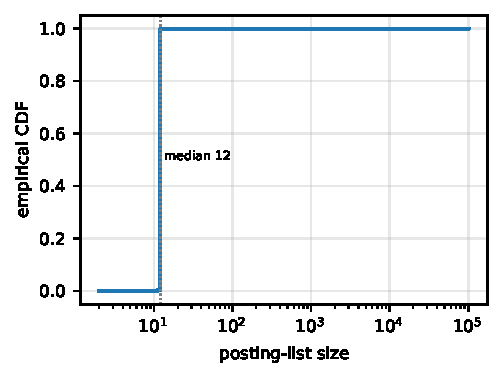
\includegraphics[width=\linewidth]{Figures/beijing/fig_posting_cdf.pdf}
\caption{Posting-list size CDF, second corpus. Flatter than the primary
corpus (Fig.~\ref{fig:postcdf}): median $12$ against $35$.}
\label{fig:postcdfbeijing}
\end{figure}

\begin{figure}[pos=t]
\centering
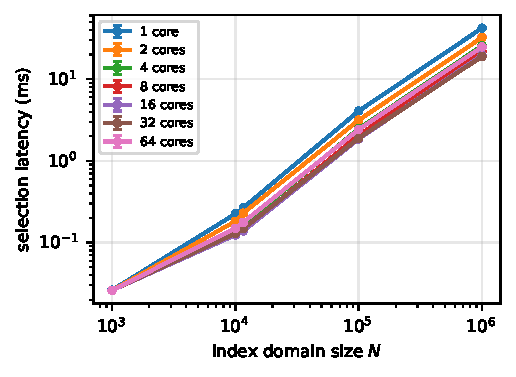
\includegraphics[width=\linewidth]{Figures/telemetry/fig_selection_latency.pdf}
\caption{Selection latency against $N$ at several thread counts. Medians of
21 runs; error bars are the interquartile range.}
\label{fig:searchlat}
\end{figure}

\begin{figure}[pos=t]
\centering
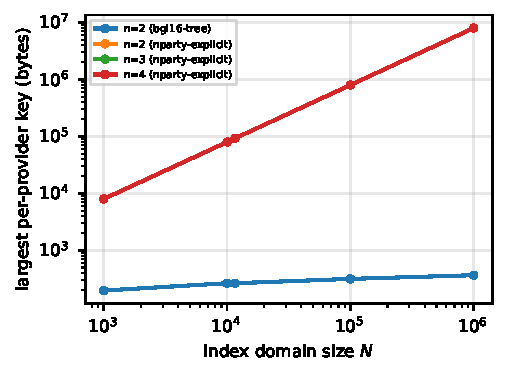
\includegraphics[width=\linewidth]{Figures/telemetry/fig_key_size.pdf}
\caption{Largest per-provider DPF key against $N$, for the two-party tree
and the non-succinct $n$-party instantiation.}
\label{fig:comm}
\end{figure}

\begin{figure}[pos=t]
\centering
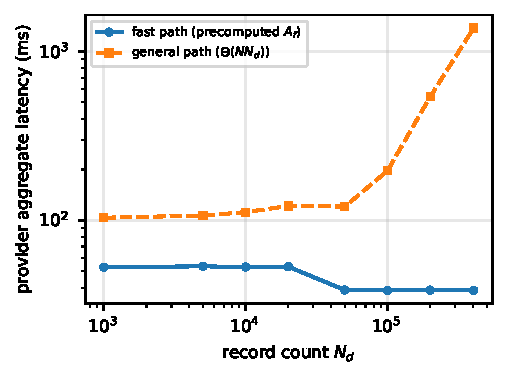
\includegraphics[width=\linewidth]{Figures/telemetry/fig_aggregate_latency.pdf}
\caption{Aggregate latency, fast against general path. The $x$-axis is $N_d$,
not $|S|$: cost no longer depends on the matched-set size. The fast path is
flat to $\pm0.5\%$ over a $405\times$ range.}
\label{fig:complat}
\end{figure}

\begin{figure}[pos=t]
\centering
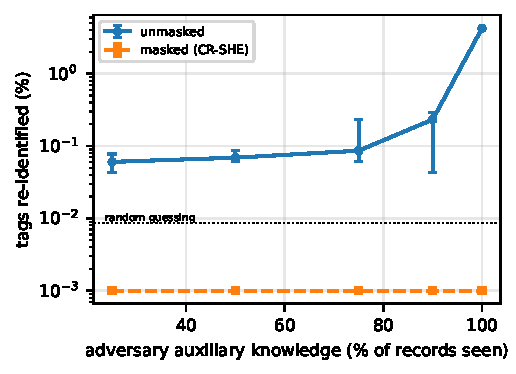
\includegraphics[width=\linewidth]{Figures/telemetry/fig_leakage_attack.pdf}
\caption{Tag re-identification against the unmasked and masked index, against
the adversary's auxiliary knowledge. Table~\ref{tab:leakage} breaks it down by
class.}
\label{fig:leakage}
\end{figure}

\begin{figure}[pos=t]
\centering
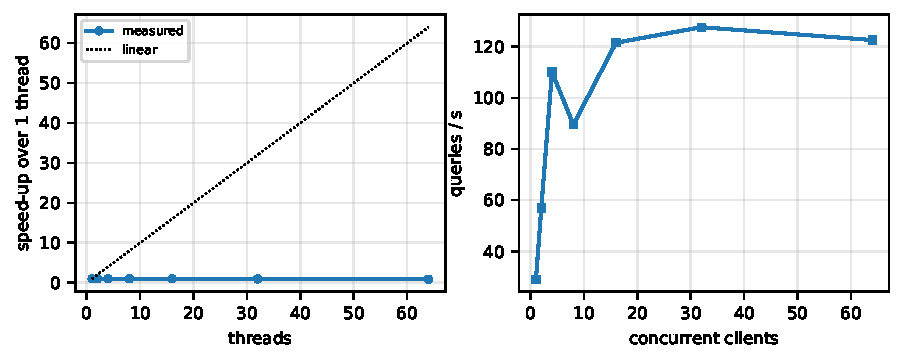
\includegraphics[width=\linewidth]{Figures/telemetry/fig_scaling.pdf}
\caption{Left: speed-up of one fast-path query with thread count. Right:
sustained throughput against concurrent clients.}
\label{fig:scaling}
\end{figure}

\begin{figure}[pos=t]
\centering
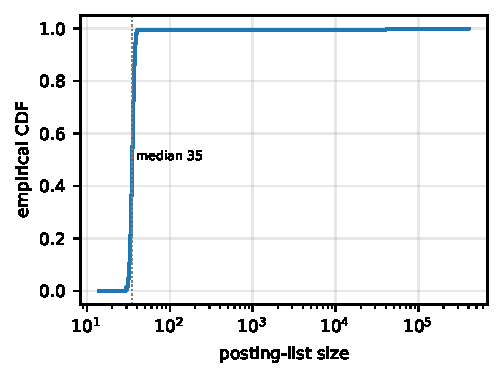
\includegraphics[width=\linewidth]{Figures/telemetry/fig_posting_cdf.pdf}
\caption{Posting-list size CDF, primary corpus. Retained to characterise the
corpus and to set the retrieval padding bound $k_{\max}$.}
\label{fig:postcdf}
\end{figure}

\subsection{Discussion}
\emph{The fast path does what it was designed to do.} Aggregate latency is
flat to $\pm0.5\%$ over a $405\times$ range of $N_d$, per-query downlink is
two ciphertexts independent of $|S|$, and provider compute is flat in $n$. A
registered single-keyword aggregate costs $3.3\times$ less than a
distributed-trust baseline that only selects and $617\times$ less than a
faithful homomorphic scan, and on the general path oblivious analytics adds
about half again to the cost of oblivious selection. Selection is linear-work
per provider on both paths; the fast path removes the dependence on record
count but restricts queries to single keywords and templates registered at
setup.

\emph{The general path is bounded by storage, not by time.} Its
$\Theta(N N_d)$ contraction reaches $1.38$\,s at the full corpus, but its
masked index is $37.5$\,GB per provider on the primary corpus and $118.2$\,GB
on the second, replicated $n$ times and resident for every query. Ad-hoc
weight vectors and conjunctions pay that price. Streaming the index from
storage in blocks would bound resident memory at the cost of I/O, though not
the work, since an aggregate needs every record's contribution; a
$\mathbb{Z}_p$ with $p<2^{32}$ would halve the index at the cost of magnitude
headroom.

\emph{Device diversity does not change the picture.} The primary corpus has
three physical devices. The twelve-site corpus, with three times the tag
domain, reproduces the per-class leakage result exactly and costs $5\%$ more
on the fast path (Section~\ref{sec:secondcorpus}).

\subsection{Limitations}
\label{sec:limits}
We collect here what the evaluation does not establish.

\emph{Deployment and hardware.} Providers ran as separate processes on one
host, so transport excludes wide-area latency, and no component was measured
on gateway-class hardware. The data user's share of the work is one DPF key
generation, $2(n-1)$ ciphertext additions and two decryptions, at
$1.4$--$1.6$\,ms on our server (Table~\ref{tab:wan}), and it is the part that
would run at the edge. Measuring it, with energy, on a gateway, and running
providers in distinct cloud regions, are the evaluations still to do.

\emph{Adversary.} Providers are semi-honest. The MAC detects inconsistent
responses except with probability $1/p$, not a consistent linear substitution
(Section~\ref{sec:verify}), and per-user query authorisation is a requirement
the prototype does not meet (Section~\ref{sec:authresult}).

\emph{Collusion beyond two providers.} For $n>2$ the prototype uses a
non-succinct sharing whose heavy key is $8N+16$ bytes, $174\times$ the
two-party key on the primary corpus. Our key-size claims are for $n=2$.

\emph{Response size.} An aggregate returns two BFV ciphertexts, $526$\,kB, for
one scalar, and $8{,}191$ of $8{,}192$ slots go unused. Switching to a smaller
ciphertext modulus before returning, and packing several templates into the
slots of one response, are standard reductions we have not applied or
measured.

\emph{Leakage baseline.} Our attack contrasts the masked index with an
unmasked one. A comparison against a padded or volume-hiding index
\citep{kamara2019computationally,patel2019mitigating} would be more demanding
and remains to be run.

\emph{Owner and ingest.} The owner retains the plaintext and rebuilds each
static tier under a fresh mask key. The prototype implements neither the
insertion of new keywords nor per-tier re-keying (Section~\ref{sec:ingest}),
and its rebuild measurement covers the fast-path columns only.

\emph{Statistical term.} Theorem~\ref{thm:mask} carries
$N N_d\,2^{-\omega}\approx2^{-31.9}$ at the prototype's $\omega=64$; sampling
mask values by rejection would remove it.

\emph{Model.} The construction assumes a single data owner and full delegation
of decryption to authorised users; multi-owner sharing and threshold or
attribute-based delegation are natural extensions. Post-quantum instantiation
follows from the lattice-based homomorphic layer for confidentiality, though
the DPF's concrete security must be revisited.

% ===========================================================================
\section{Conclusion}
\label{sec:conclusion}

This paper addressed a composition leak in distributed-trust query systems:
hiding which records a query selects is of limited value if aggregating over
them hands the selection back to the servers. CR-SHE removes that leak with
oblivious homomorphic aggregation, in which each provider contracts its own
distributed-point-function share directly against the homomorphically
encrypted record column and returns a single ciphertext, so the matched set is
never assembled at any provider and its cardinality never leaves the client. A
precomputed-column variant makes single-keyword aggregates independent of the
record count, and a one-time-pad index mask, cancelled inside the ciphertext,
removes the posting-list leakage a replicated index otherwise exposes at rest.
We proved correctness and adaptive security against a coalition of up to
$t=n-1$ providers with a per-query leakage profile revealing only the
requested aggregate class, over data encrypted under a single owner's key and
without any communication between providers. On two real IoT corpora the
prototype answers a registered single-keyword aggregate in $39$\,ms per
provider, independently of the record count and of the matched-set size,
which places end-to-end obliviousness within reach of a multi-cloud IoT
deployment rather than beyond it. Future work will pursue sublinear
preprocessing, verification and authorisation proofs compatible with
non-interacting providers, a wide-area multi-cloud and edge-hardware
evaluation, multi-owner multi-key deployment, and richer predicates than
single-keyword selection.

% ===========================================================================
% \printcredits emits its own "CRediT authorship contribution statement"
% heading from the \credit declarations in the front matter.
\printcredits

\section*{Declaration of competing interest}
The authors declare that they have no known competing financial interests or
personal relationships that could have appeared to influence the work reported
in this paper.

\section*{Declaration of generative AI and AI-assisted technologies in the
writing process}
The authors did not use generative AI or AI-assisted technologies in the
preparation of this work beyond routine language and grammar checking, and
they reviewed and edited the content as needed and take full responsibility
for the content of the published article.

% ===========================================================================
\bibliographystyle{model1-num-names}
\bibliography{references}

\end{document}
